\chapter{Examples}

\section{Receptor phosphorylation}

\begin{figure}[H]
\begin{center}
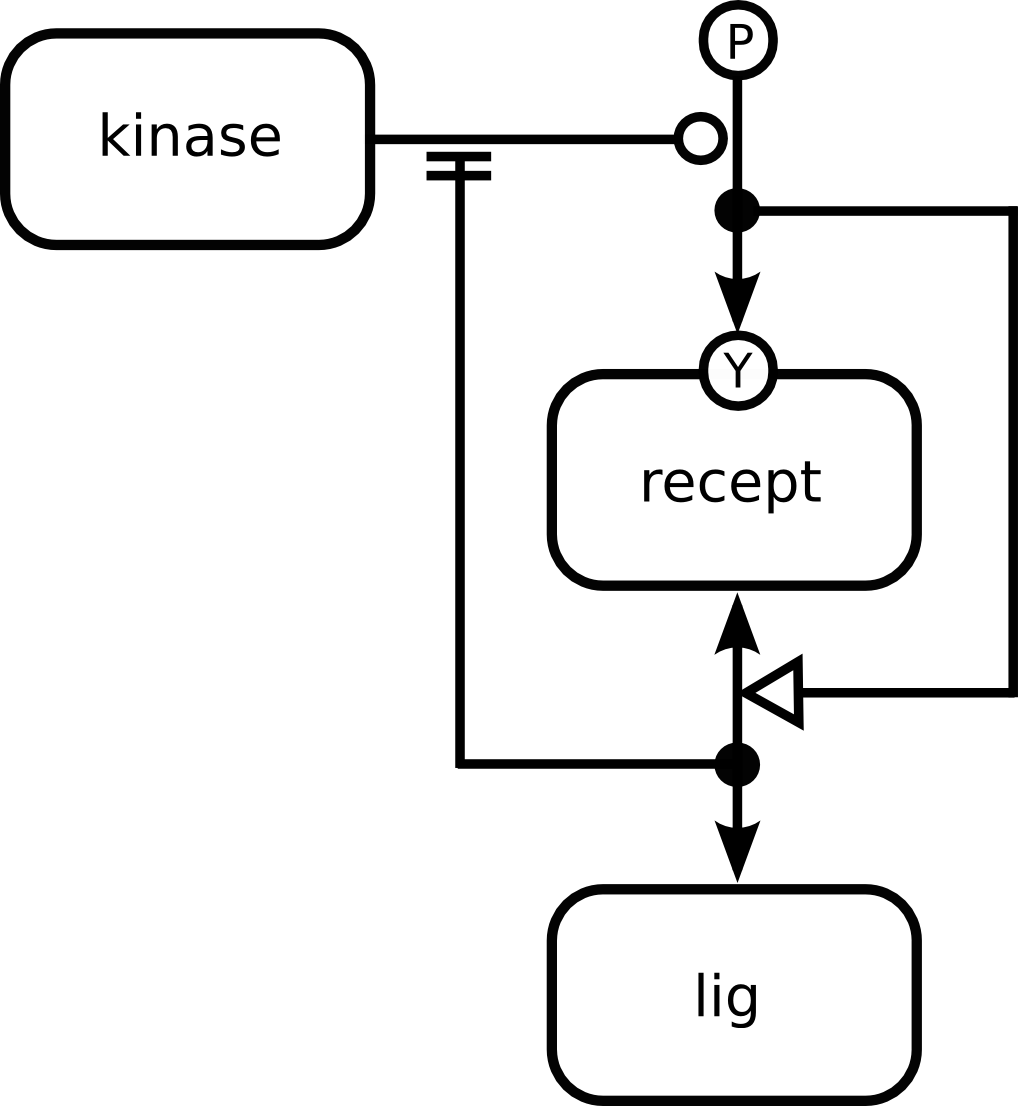
\includegraphics{figs/pngs/example_phospho_receptor.png}
\caption{A receptor can bind a ligand, and be phosphorylated by a kinase. The phosphorylation can only take place on the free receptor. The binding reaction is stimulated by the phosphorylation. The figure is drawn using the SBGN Entity Relationship language.}
\label{fig:receptor}
\end{center}
\end{figure}

\begin{example}
<?xml version="1.0" encoding="UTF-8"?>
<sbml xmlns="http://www.sbml.org/sbml/level3/version1/core" level="3" version="1"
      xmlns:multi="http://www.sbml.org/sbml/level3/version1/multi/version1"
      multi:required="true">

  <model name="phosphoreceptor">

    <listOfCompartments>
      <compartment id="cell" constant="true" size="1" />
    </listOfCompartments>

<!-- -------------------------------------------------------------------------------- -->
<!-- We need to define two species types to be able to describe all the reactions.    -->
<!-- There is not species type for the kinase, that is not used in selectors.         -->
<!-- -------------------------------------------------------------------------------- -->

    <multi:listOfSpeciesTypes>
    
      <multi:speciesType multi:id="st_recept" 
                         multi:name="receptor" 
                         multi:bindingSite="true">
        <multi:listOfStateFeatures>
          <multi:stateFeature multi:id="Y" multi:name="tyrosine">
            <multi:listOfPossibleValues>      
              <multi:possibleValue multi:id="P" multi:name="phosphorylated" />
              <multi:possibleValue multi:id="nonP" multi:name="nonphosphorylated" />
            </multi:listOfPossibleValues>
          </multi:stateFeature>
        </multi:listOfStateFeatures>
      </multi:speciesType>
      
      <multi:speciesType multi:id="st_lig" multi:name="ligand" multi:bindingSite="true" />
    </multi:listOfSpeciesTypes>

    <multi:listOfSelectors>
\end{example}

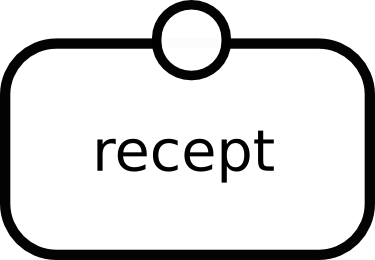
\includegraphics{figs/pngs/sel_freereceptor_nonP.png}

\begin{example}
<!-- -------------------------------------------------------------------------------- -->
<!-- Description of receptor, unbound, unphosphorylated                               -->
<!-- -------------------------------------------------------------------------------- -->
    
      <multi:selector multi:id="sel_freereceptor_nonP">
        <multi:listOfSpeciesTypeStates>
          <multi:speciesTypeState multi:id="sts_recept" multi:speciesType="st_recept" 
                                   multi:minOccur="1" multi:maxOccur="1">
            <multi:listOfStateFeatureInstances>
              <multi:stateFeatureInstance multi:stateFeature="Y">
                <multi:stateFeatureValue multi:possibleValue="nonphosphorylated" />
              </multi:stateFeatureInstance>
            </multi:listOfStateFeatureInstances>
          </multi:speciesTypeState>
        </multi:listOfSpeciesTypeStates>
        <multi:listOfUnboundBindingSites>
          <multi:bindingSiteReference multi:speciesTypeState="sts_recept" />
        </multi:listOfUnboundBindingSites>
      </multi:selector>
\end{example}

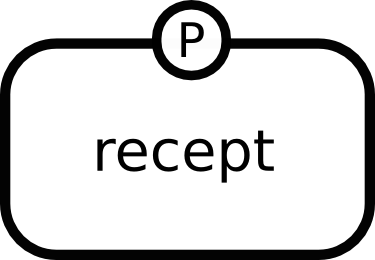
\includegraphics{figs/pngs/sel_freereceptor_P.png}

\begin{example}
<!-- -------------------------------------------------------------------------------- -->
<!-- Description of receptor, unbound, phosphorylated                                 -->
<!-- -------------------------------------------------------------------------------- -->
      <multi:selector multi:id="sel_freereceptor_P">
        <multi:listOfSpeciesTypeStates>
          <multi:speciesTypeState multi:id="sts_recept" multi:speciesType="st_recept" 
                                   multi:minOccur="1" multi:maxOccur="1">
            <multi:listOfStateFeatureInstances>
              <multi:stateFeatureInstance multi:stateFeature="Y">
                <multi:stateFeatureValue multi:possibleValue="phosphorylated" />
              </multi:stateFeatureInstance>
            </multi:listOfStateFeatureInstances>
          </multi:speciesTypeState>
        </multi:listOfSpeciesTypeStates>
        <multi:listOfUnboundBindingSites>
          <multi:bindingSiteReference multi:speciesTypeState="sts_recept" />
        </multi:listOfUnboundBindingSites>
      </multi:selector>
\end{example}

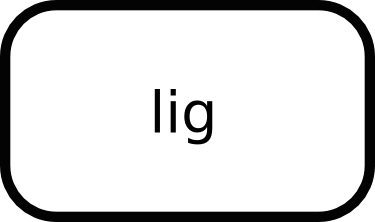
\includegraphics{figs/pngs/sel_freeligand.png}

\begin{example}
<!-- -------------------------------------------------------------------------------- -->
<!-- Description of ligand, unbound                                                   -->
<!-- -------------------------------------------------------------------------------- -->
      <multi:selector multi:id="sel_freeligand">
        <multi:listOfSpeciesTypeStates>
          <multi:speciesTypeState multi:id="sts_lig" multi:speciesType="st_lig" 
                                   multi:minOccur="1" multi:maxOccur="1" />
        </multi:listOfSpeciesTypeStates>
        <multi:listOfUnboundBindingSites>
          <multi:bindingSiteReference multi:speciesTypeState="sts_lig" />
        </multi:listOfUnboundBindingSites>
      </multi:selector>
\end{example}

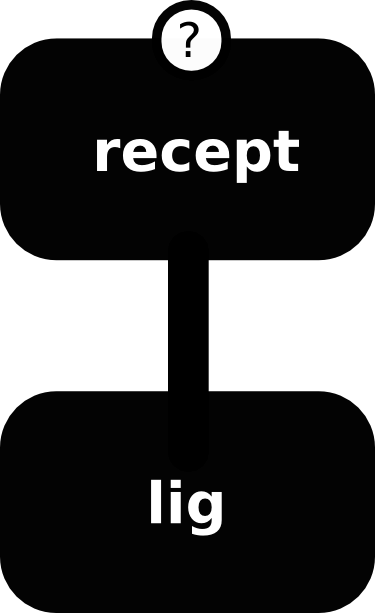
\includegraphics{figs/pngs/sel_complex.png}

\begin{example}
<!-- -------------------------------------------------------------------------------- -->
<!-- Description of the ligand-receptor complex                                       -->
<!-- -------------------------------------------------------------------------------- -->      
      <multi:selector multi:id="sel_complex">
        <multi:listOfSpeciesTypeStates>
          <multi:speciesTypeState multi:id="sts_recept" multi:speciesType="st_recept" 
                                   multi:minOccur="1" multi:maxOccur="1" />
          <multi:speciesTypeState multi:id="sts_lig" multi:speciesType="st_lig" 
                                   multi:minOccur="1" multi:maxOccur="1" />
        </multi:listOfSpeciesTypeStates>
        <multi:listOfBonds>
          <multi:bond multi:occurrence="required">
            <multi:bindingSiteReference multi:speciesTypeState="sts_lig" />
            <multi:bindingSiteReference multi:speciesTypeState="sts_recept" />
          </multi:bond>
        </multi:listOfBonds>
      </multi:selector>
      
    </multi:listOfSelectors>

    <listOfSpecies>
      <species id="kinase" compartment="cell" boundaryCondition="false" 
               hasOnlySubstanceUnit="false" constant="false" initialAmount="100" />
      <species id="recept" compartment="cell" multi:speciesType="st_recept" 
               boundaryCondition="false" hasOnlySubstanceUnit="false" 
               constant="false" initialAmount="100" >
        <multi:listOfSpeciesTypeInstances>
          <multi:SpeciesTypeInstance multi:id="freereceptor_nonP" 
                                     multi:initialAmount="100">
            <multi:listOfSelectorReferences>
              <multi:selectorReference multi:selector="sel_freereceptor_nonP" />
            </multi:listOfSelectorReferences>
          </multi:speciesTypeInstance>
          <multi:SpeciesTypeInstance multi:id="freereceptor_P" 
                                     multi:initialAmount="0">
            <multi:listOfSelectorReferences>
              <multi:selectorReference multi:selector="sel_freereceptor_P" />
            </multi:listOfSelectorReferences>
          </multi:speciesTypeInstance>
          <multi:SpeciesTypeInstance multi:id="boundreceptor">
            <multi:listOfSelectorReferences>
              <multi:selectorReference multi:selector="sel_complex">
            </multi:listOfSelectorReferences>
          </multi:speciesTypeInstance>
        </multi:listOfSpeciesTypeInstances>
      </species>
      <species id="lig" compartment="cell" multi:speciesType="st_lig" 
                       boundaryCondition="false" 
               hasOnlySubstanceUnit="false" constant="false" initialAmount="1000" >
        <multi:listOfSpeciesTypeInstances>
          <multi:SpeciesTypeInstance multi:id="freeligand" multi:initialAmount="1000">
            <multi:listOfSelectorReferences>
              <multi:selectorReference multi:selector="sel_freeligand" />
            </multi:listOfSelectorReferences>
          </multi:speciesTypeInstance>
          <multi:SpeciesTypeInstance multi:id="boundligand" multi:initialAmount="0">
            <multi:listOfSelectorReferences>
              <multi:selectorReference multi:selector="sel_complex">
            </multi:listOfSelectorReferences>
          </multi:speciesTypeInstance>
        </multi:listOfSpeciesTypeInstances>
      </species>
    </listOfSpecies>

    <listOfReactions>
\end{example}

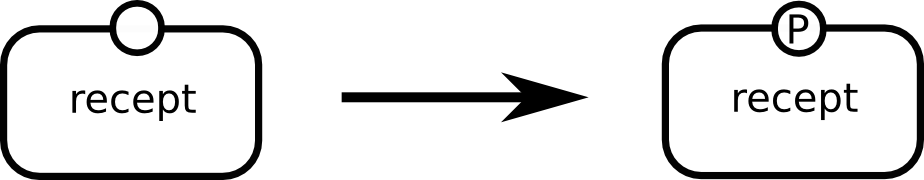
\includegraphics{figs/pngs/ReceptPhosphorylation.png}

\begin{example}
<!-- -------------------------------------------------------------------------------- -->
<!-- Phosphorylation of the receptor by the kinase when unbound                        -->
<!-- -------------------------------------------------------------------------------- -->      
     
      <reaction id="phosphorylation" reversible="false" fast="false">
        <listOfReactants>
          <speciesReference species="recept" stoichiometry="1">
            <multi:listOfSpeciesRestriction>
              <multi:speciesRestriction multi:id="freeRnonP" 
                                        multi:speciesTypeInstance="freereceptor_nonP" />
            </multi:listOfSpeciesRestriction>
          </speciesReference>
        </listOfReactants>
        <listOfProducts>
          <multi:productSpeciesReference species="recept" stoichiometry="1">
            <multi:listOfSpeciesRestriction>
              <multi:speciesRestriction multi:id="freeRP" 
                                        multi:speciesTypeInstance="freereceptor_P" />
            </multi:listOfSpeciesRestriction>
          </multi:productSpeciesReference>
        </listOfProducts>
        <listOfModifiers>
          <modifierSpeciesReference species="kinase" />
        </listOfModifiers>
        <kineticLaw>
          <math xmlns="http://www.w3.org/1998/Math/MathML" />
        </kineticLaw>
        <multi:listOfReactionRules>
          <multi:reactionRule multi:id="PhosphorylationUnbound">
            <multi:listOfConditions>
              <multi:speciesTypeRestrictionReference multi:speciesTypeRestriction="freeRnonP"/>
            </multi:listOfConditions>
            <multi:listOfResults>
              <multi:speciesTypeRestrictionReference multi:speciesTypeRestriction="freeRP"/>
            </multi:listOfResults>
            <kineticLaw>
              <math xmlns="http://www.w3.org/1998/Math/MathML" >
                <apply>
                  <times />
                  <ci> cell </ci>
                  <ci> Vm </ci>
                  <apply>
                    <divide />
                    <ci> recept </ci>
                    <apply>
                      <plus />
                      <ci> recept </ci>
                      <ci> Km </ci>
                    </apply>
                  </apply>
                </apply>
              </math>
              <listOfLocalParameters>
                <localParameter id="Km" value="1" />
                <localParameter id="Vm" value="1" />
              </listOfLocalParameters>
             </kineticLaw>
          </multi:reactionRule>
        </multi:listOfReactionRules>

      </reaction>
\end{example}

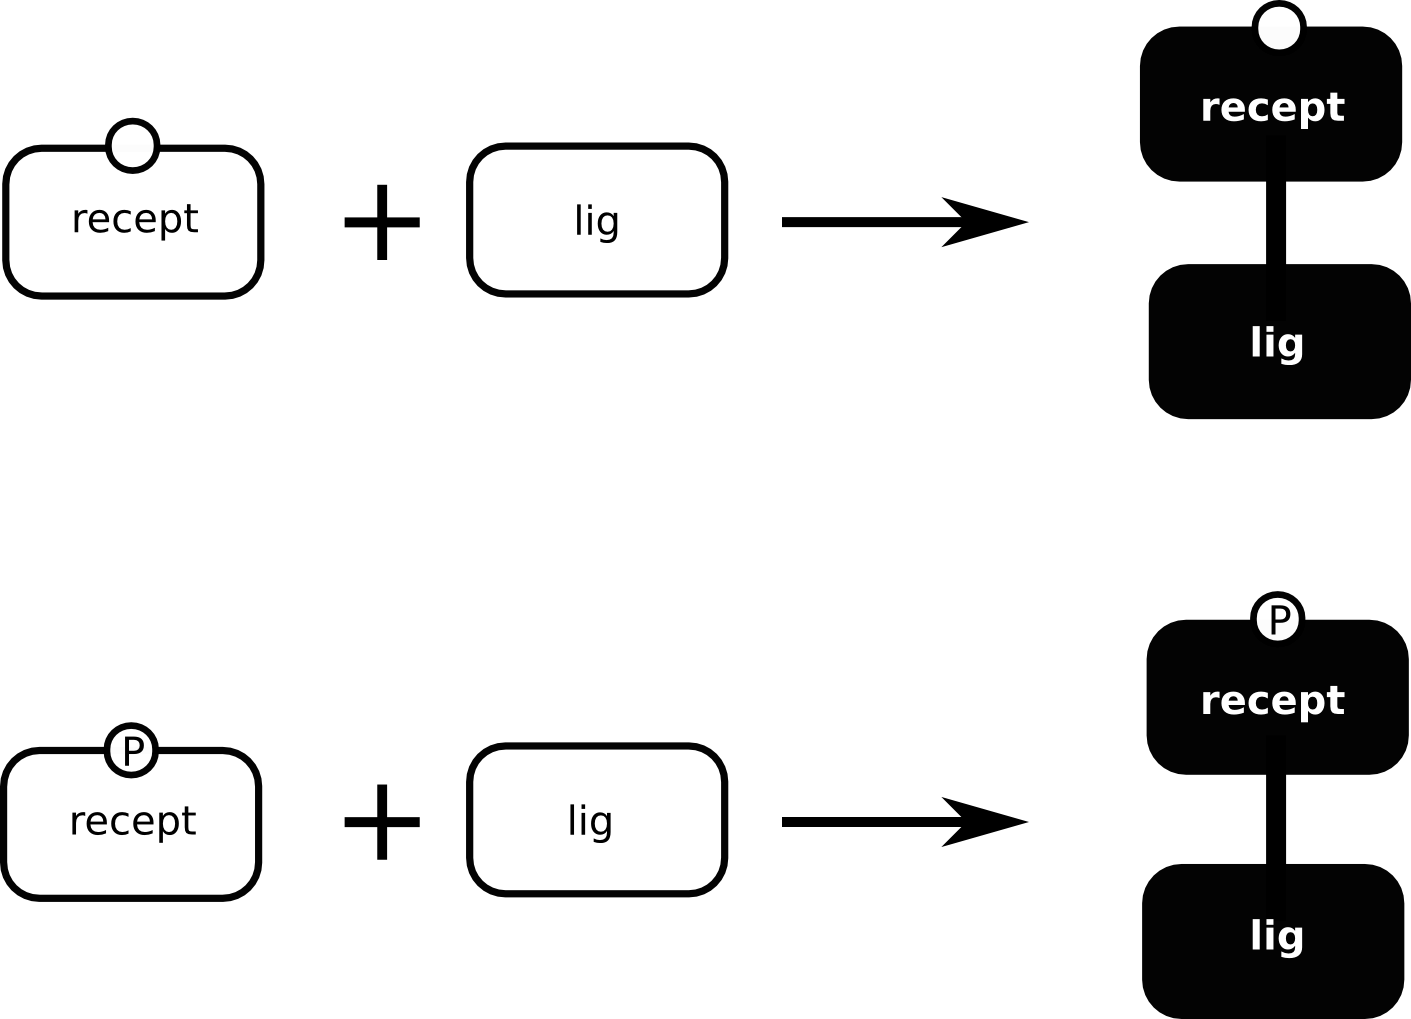
\includegraphics{figs/pngs/receptLigBinding.png}

\begin{example}
<!-- -------------------------------------------------------------------------------- -->
<!-- Ligand binding, when the receptor is phosphorylated or not                       -->
<!-- -------------------------------------------------------------------------------- -->      
       
      <reaction id="receptLigBinding" reversible="false" fast="false"> 
        <listOfReactants>
          <speciesReference id="react_recept" species="recept" stoichiometry="1">
            <multi:listOfSpeciesRestriction>
              <multi:speciesRestriction multi:id="freeRnonP" 
                                        multi:speciesTypeInstance="freereceptor_nonP" />
              <multi:speciesRestriction multi:id="freeRP" 
                                        multi:speciesTypeInstance="freereceptor_P" />
            </multi:listOfSpeciesRestriction>
          </speciesReference>
          <speciesReference id="react_lig" species="lig" stoichiometry="1">
            <multi:listOfSpeciesRestriction>
              <multi:speciesRestriction multi:id="freeL" 
                                        multi:speciesTypeInstance="freeligand" />
            </multi:listOfSpeciesRestriction>
          </speciesReference>
        </listOfReactants>
        <listOfProducts>
          <multi:productSpeciesReference species="recept" stoichiometry="1"
                                   correspondingReactant="react_recept">
            <multi:listOfSpeciesRestriction>
              <multi:speciesRestriction multi:id="boundR" 
                                        multi:speciesTypeInstance="boundreceptor" />
            </multi:listOfSpeciesRestriction>
          </multi:productSpeciesReference>
          <multi:productSpeciesReference species="lig" stoichiometry="1"
                                   correspondingReactant="react_lig">
            <multi:listOfSpeciesRestriction>
              <multi:speciesRestriction multi:id="boundL" 
                                        multi:speciesTypeInstance="boundligand" />
            </multi:listOfSpeciesRestriction>
          </multi:productSpeciesReference>
        </listOfProducts>
        <kineticLaw>
          <math xmlns="http://www.w3.org/1998/Math/MathML" />
        </kineticLaw>
        <multi:listOfReactionRules>
          <multi:reactionRule multi:id="bindingNonPhospho">
            <multi:listOfConditions>
              <multi:speciesTypeRestrictionReference multi:speciesTypeRestriction="freeRnonP" />
              <multi:speciesTypeRestrictionReference multi:speciesTypeRestriction="freeL" />
            </multi:listOfConditions>
            <multi:listOfResults>
              <multi:speciesTypeRestrictionReference multi:speciesTypeRestriction="boundR" />
              <multi:speciesTypeRestrictionReference multi:speciesTypeRestriction="boundL" />
            </multi:listOfResults>
            <kineticLaw>
              <math xmlns="http://www.w3.org/1998/Math/MathML" >
                <apply>
                  <times />
                  <ci> cell </ci>
                  <ci> kon_nonphos </ci>
                  <ci> recept </ci>
                  <ci> lig </ci>
                </apply>
              </math>
              <listOfLocalParameters>
                <localParameter id="kon_nonphos" value="1">
              </listOfLocalParameters>
            </kineticLaw>
          </multi:reactionRule>
          <multi:reactionRule multi:id="bindingPhospho">
            <multi:listOfConditions>
              <multi:speciesTypeRestrictionReference multi:speciesTypeRestriction="freeRP" />
              <multi:speciesTypeRestrictionReference multi:speciesTypeRestriction="freeL" />
            </multi:listOfConditions>
            <multi:listOfResults>
              <multi:speciesTypeRestrictionReference multi:speciesTypeRestriction="boundR" />
              <multi:speciesTypeRestrictionReference multi:speciesTypeRestriction="boundL" />
            </multi:listOfResults>

            <kineticLaw>
              <math xmlns="http://www.w3.org/1998/Math/MathML" >
                <apply>
                  <times />
                  <ci> cell </ci>
                  <ci> kon_phos </ci>
                  <ci> recept </ci>
                  <ci> lig </ci>
                </apply>
              </math>
              <listOfLocalParameters>
                <localParameter id="kon_phos" value="10">
              </listOfLocalParameters>
            </kineticLaw>
          </multi:reactionRule>
        </multi:listOfReactionRules>
      </reaction>
    </listOfReactions>

  </model>
</sbml>
\end{example}

\section{Microtubule polymerisation}

\begin{figure}[H]
\begin{center}
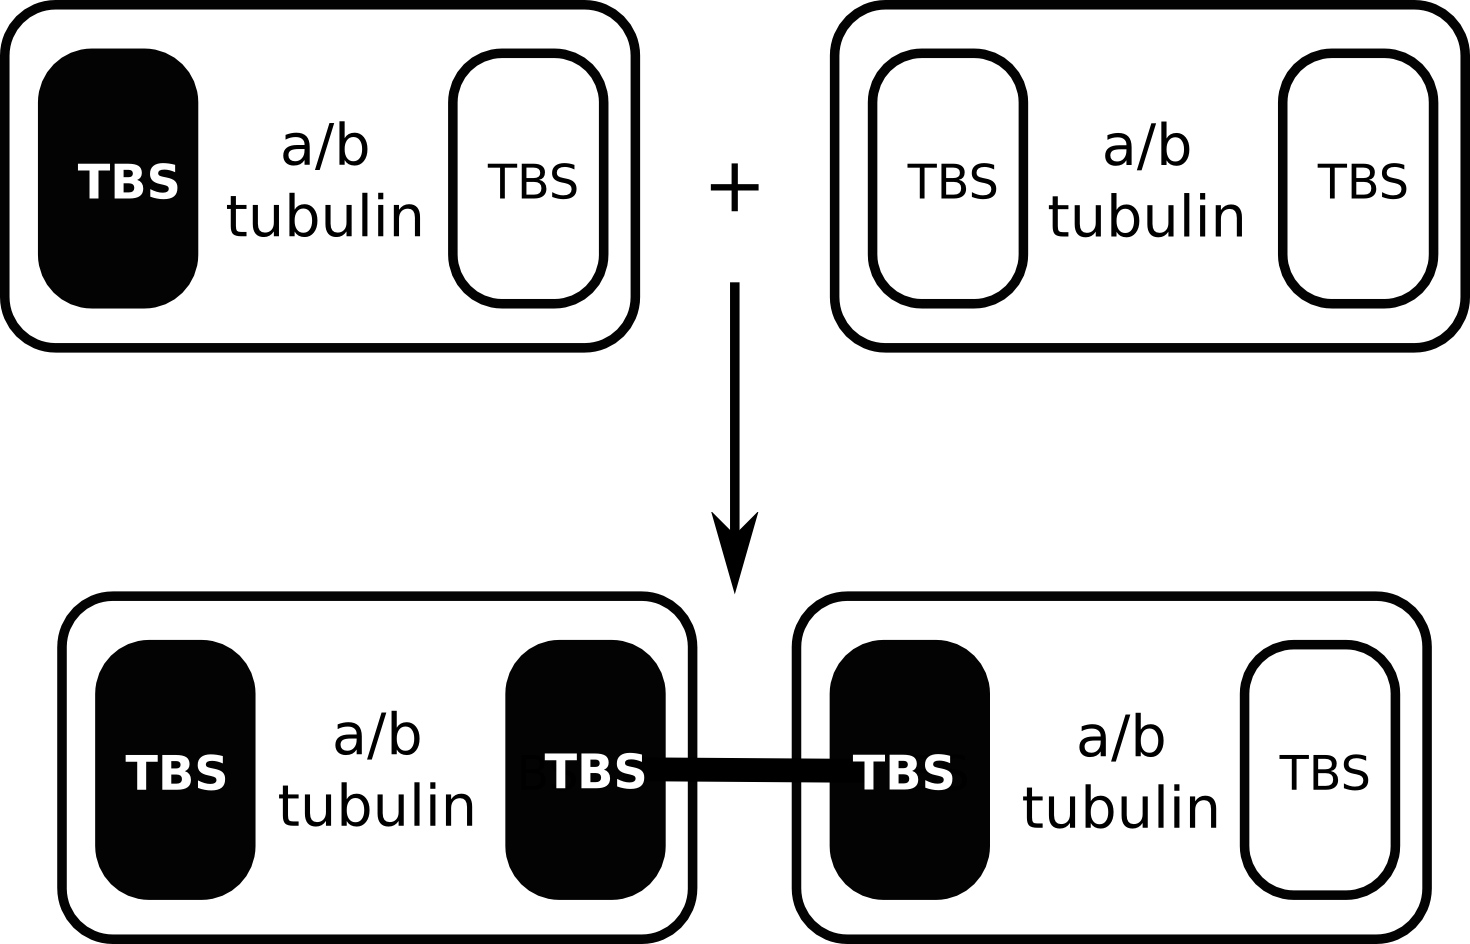
\includegraphics{figs/pngs/microtubule.png}
\caption{A microtubule of undefined length can be extended through a polimerization reaction.}
\label{fig:microtubule2}
\end{center}
\end{figure}

Within the context of the example detailed below, where only microtubules and tubulin dimers can bind, the figure \ref{fig:microtubule2} is effectively equivalent to the figure \label{fig:microtubule3}, both representing the same reactions.

\begin{figure}[H]
\begin{center}
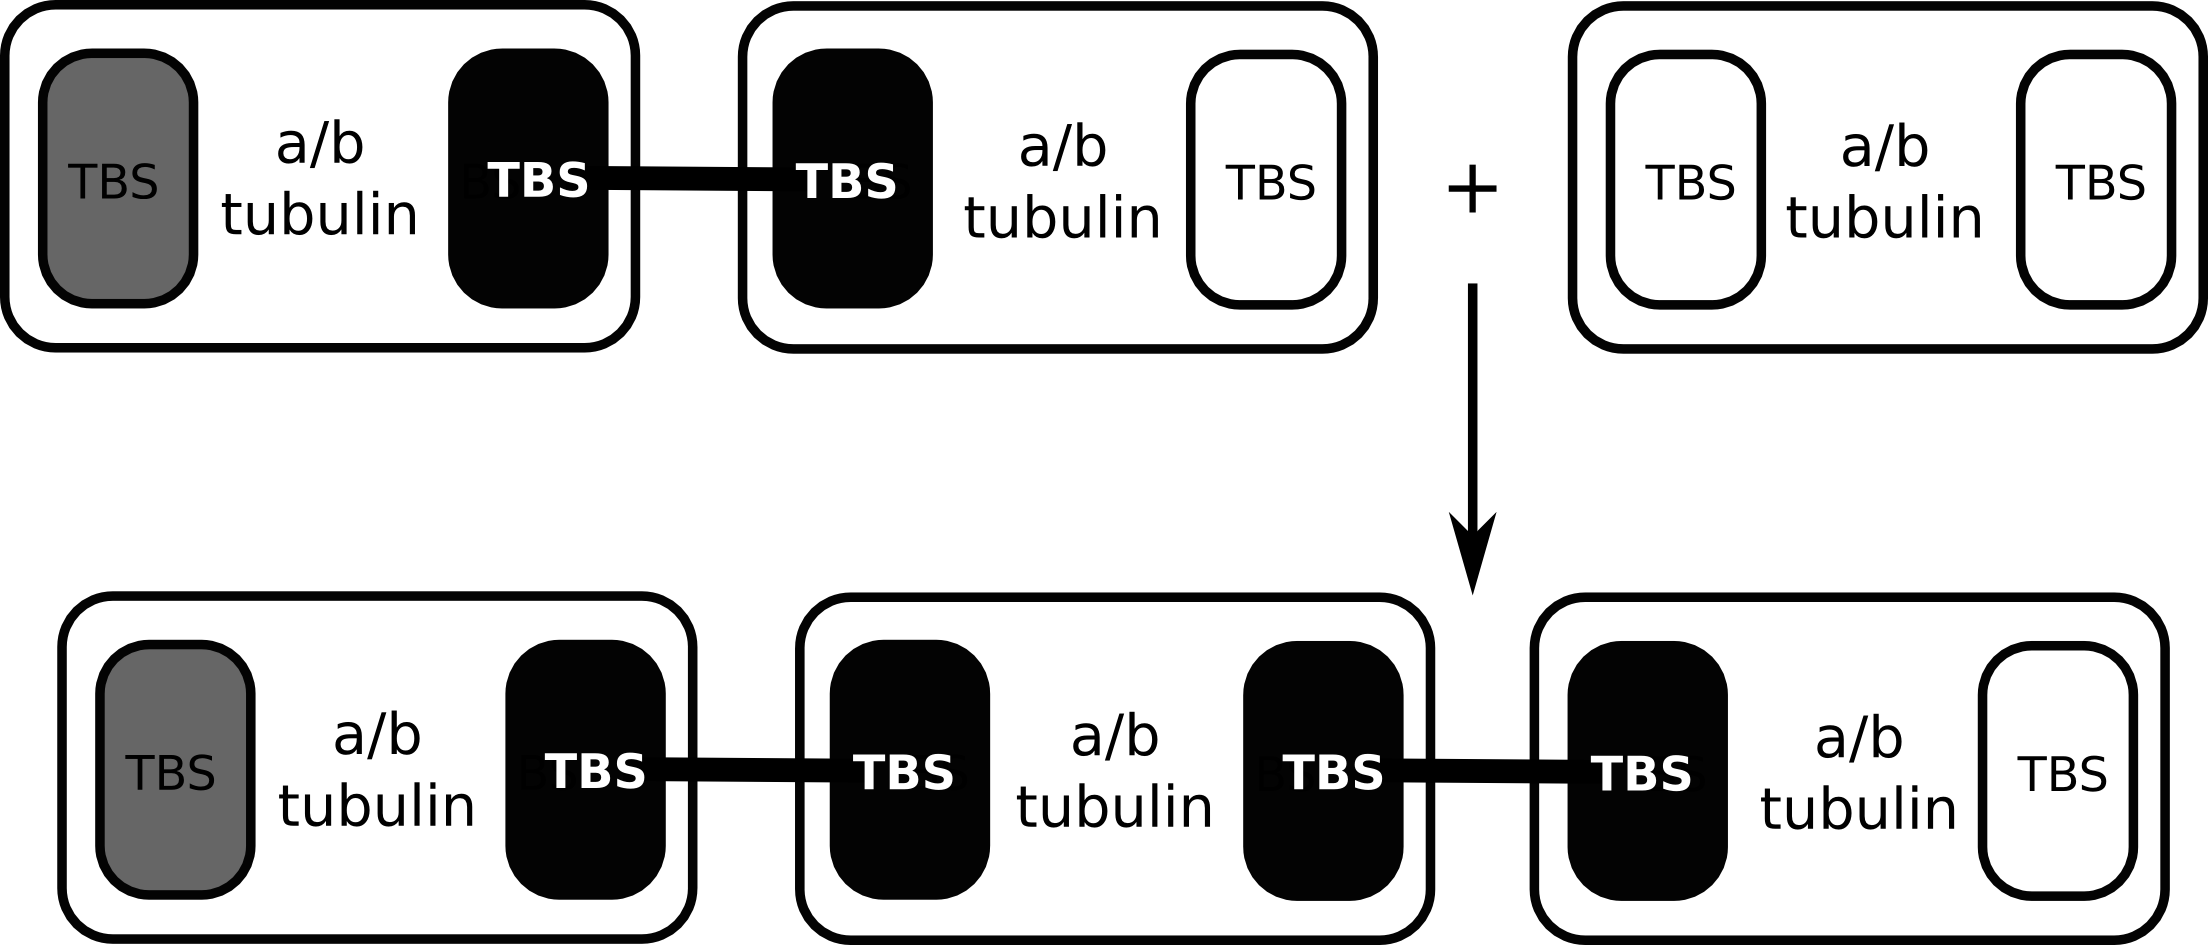
\includegraphics{figs/pngs/microtubule-alt.png}
\caption{A microtubule of undefined length can be extended through a polimerization reaction.}
\label{fig:microtubule3}
\end{center}
\end{figure}

\begin{example}
<?xml version="1.0" encoding="UTF-8"?>
<sbml xmlns="http://www.sbml.org/sbml/level3/version1/core" level="3" version="1"
      xmlns:multi="http://www.sbml.org/sbml/level3/version1/multi/version1"
      multi:required="true">

  <model name="microtubule_elongation">

    <listOfCompartments>
      <compartment id="cell" constant="true" size="1" />
    </listOfCompartments>

    <multi:listOfSpeciesTypes>
    
      <multi:speciesType multi:id="st_tubulin" multi:name="tubulin" multi:bindingSite="false">
      <multi:speciesType multi:id="st_tbs" multi:name="tbs" multi:bindingSite="true" />
    
    </multi:listOfSpeciesTypes>

    <multi:listOfSelectors>
\end{example}

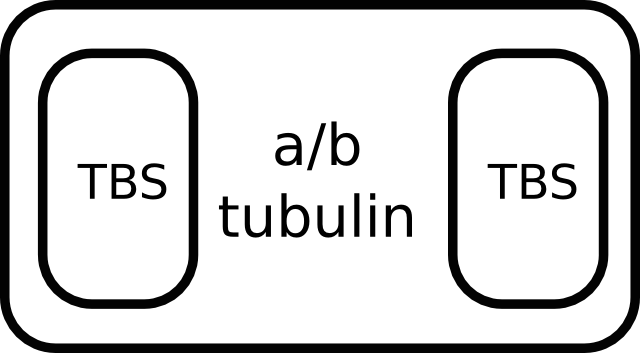
\includegraphics{figs/pngs/sel_tubulin_free.png}

\begin{example}
<!-- -------------------------------------------------------------------------------- -->
<!-- Description of a free dimer of tubulin                                           -->
<!-- -------------------------------------------------------------------------------- -->
    
      <multi:selector multi:id="sel_tubulin_free">
        <multi:listOfSpeciesTypeStates>
          <multi:speciesTypeState multi:id="sts_tbs1" multi:speciesType="st_tbs" 
                                   multi:minOccur="1" multi:maxOccur="1" />
          <multi:speciesTypeState multi:id="sts_tbs2" multi:speciesType="st_tbs" 
                                   multi:minOccur="1" multi:maxOccur="1" />
          <multi:speciesTypeState multi:id="sts_tubulin" multi:speciesType="st_tubulin" 
                                   multi:minOccur="1" multi:maxOccur="1" />
            <multi:listOfContainedSpeciesTypes>
              <multi:containedSpeciesType multi:speciesTypeState="sts_tbs1" /> 
              <multi:containedSpeciesType multi:speciesTypeState="sts_tbs2" />
            </multi:listOfContainedSpeciesTypes>
          </multi:speciesTypeStates>
        </multi:listOfSpeciesTypeStates>
        <multi:listOfUnboundBindingSites>
          <multi:bindingSiteReference multi:speciesTypeState="sts_tbs1" />
          <multi:bindingSiteReference multi:speciesTypeState="sts_tbs2" />
        </multi:listOfUnboundBindingSites>
      </multi:selector>
\end{example}

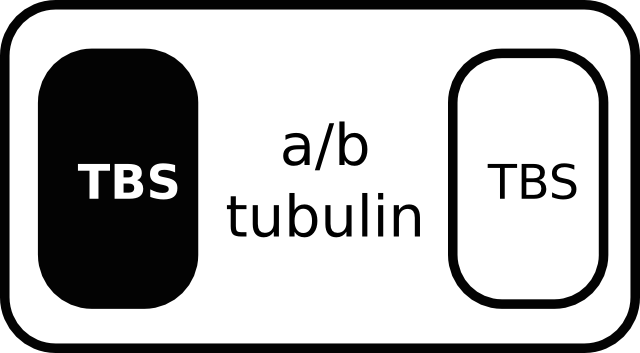
\includegraphics{figs/pngs/sel_microtubule.png}

\begin{example}
<!-- -------------------------------------------------------------------------------- -->
<!-- To signify a microtubule, we describe a tubulin with one binding site free, the  -->
<!-- other being bound                                                                -->
<!-- -------------------------------------------------------------------------------- -->
      <multi:selector multi:id="sel_microtubule">
        <multi:listOfSpeciesTypeStates>
          <multi:speciesTypeState multi:id="sts_tbs1" multi:speciesType="st_tbs" 
                                   multi:minOccur="1" multi:maxOccur="1" />
          <multi:speciesTypeState multi:id="sts_tbs2" multi:speciesType="st_tbs" 
                                   multi:minOccur="1" multi:maxOccur="1" />
          <multi:speciesTypeState multi:id="sts_tubulin" multi:speciesType="st_tubulin" 
                                   multi:minOccur="1" multi:maxOccur="1" />
            <multi:listOfContainedSpeciesTypes>
              <multi:containedSpeciesType multi:speciesTypeState="sts_tbs1" /> 
              <multi:containedSpeciesType multi:speciesTypeState="sts_tbs2" />
            </multi:listOfContainedSpeciesTypes>
          </multi:speciesTypeStates>
        </multi:listOfSpeciesTypeStates>
        <multi:listOfUnboundBindingSites>
          <multi:bindingSiteReference multi:speciesTypeState="sts_tbs1" />
        </multi:listOfUnboundBindingSites>
        <multi:listOfBonds>
          <multi:bond multi:occurrence="required" >
            <multi:bindingSiteReference multi:speciesTypeState="sts_tbs2" />
          </multi:bond>
        </multi:listOfBonds>
      </multi:selector>

\end{example}

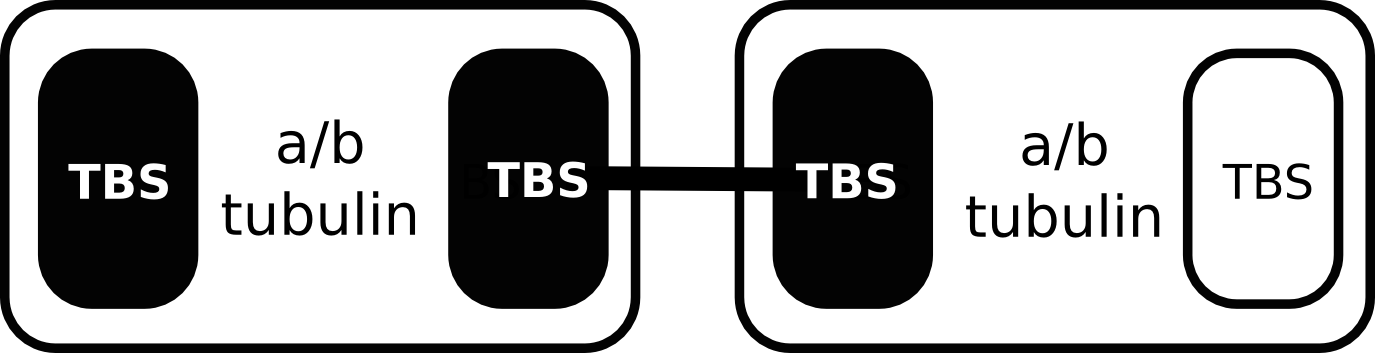
\includegraphics{figs/pngs/sel_microtubuleExtended.png}

\begin{example}
<!-- -------------------------------------------------------------------------------- -->
<!-- This is a microtubule with at least three monomers                               -->
<!-- -------------------------------------------------------------------------------- -->
      <multi:selector multi:id="sel_microtubuleExtended">
        <multi:listOfSpeciesTypeStates>
          <multi:speciesTypeState multi:id="sts_tbs1" multi:speciesType="st_tbs" 
                                   multi:minOccur="1" multi:maxOccur="1" />
          <multi:speciesTypeState multi:id="sts_tbs2" multi:speciesType="st_tbs" 
                                   multi:minOccur="1" multi:maxOccur="1" />
          <multi:speciesTypeState multi:id="sts_tbs3" multi:speciesType="st_tbs" 
                                   multi:minOccur="1" multi:maxOccur="1" />
          <multi:speciesTypeState multi:id="sts_tbs4" multi:speciesType="st_tbs" 
                                   multi:minOccur="1" multi:maxOccur="1" />
          <multi:speciesTypeState multi:id="sts_tubulin1" multi:speciesType="st_tubulin" 
                                   multi:minOccur="1" multi:maxOccur="1">
            <multi:listOfContainedSpeciesTypes>
              <multi:containedSpeciesType multi:speciesTypeState="sts_tbs1" /> 
              <multi:containedSpeciesType multi:speciesTypeState="sts_tbs2" />
            </multi:listOfContainedSpeciesTypes>
          </multi:speciesTypeStates>
          <multi:speciesTypeStates multi:id="sts_tubulin2" multi:speciesType="st_tubulin" 
                                   multi:minOccur="1" multi:maxOccur="1">
            <multi:listOfContainedSpeciesTypes>
              <multi:containedSpeciesType multi:speciesTypeState="sts_tbs3" /> 
              <multi:containedSpeciesType multi:speciesTypeState="sts_tbs4" />
            </multi:listOfContainedSpeciesTypes>
          </multi:speciesTypeStates>
        </multi:listOfSpeciesTypeStates>
        <multi:listOfBonds>
          <multi:bond multi:occurrence="required" >
            <multi:bindingSiteReference multi:speciesTypeState="sts_tbs2" />
            <multi:bindingSiteReference multi:speciesTypeState="sts_tbs3" />
          </multi:bond>
        </multi:listOfBonds>
        <multi:listOfUnboundBindingSites>
          <multi:bindingSiteReference multi:speciesTypeState="sts_tbs1" />
        </multi:listOfUnboundBindingSites>
      </multi:selector>
    </multi:listOfSelectors>

    <listOfSpecies>
      <species id="tubulin" compartment="cell" multi:speciesType="st_tubulin"
               boundaryCondition="false" hasOnlySubstanceUnit="false" 
               constant="false" initialAmount="500" >
        <multi:listOfSpeciesTypeInstances>
          <multi:SpeciesTypeInstance multi:id="free_tubulin" multi:initialAmount="100">
            <multi:listOfSelectorReferences>
              <multi:selectorReference multi:selector="sel_tubulin_free" />
            </multi:listOfSelectorReferences>
          </multi:speciesTypeInstance>
          <multi:SpeciesTypeInstance multi:id="microtubule" multi:initialAmount="400">
            <multi:listOfSelectorReferences>
              <multi:selectorReference multi:selector="sel_microtubule" />
            </multi:listOfSelectorReferences>
          </multi:speciesTypeInstance>
          <multi:SpeciesTypeInstance multi:id="microtubuleExtended" multi:initialAmount="0">
            <multi:listOfSelectorReferences>
              <multi:selectorReference multi:selector="sel_microtubuleExtended">
            </multi:listOfSelectorReferences>
          </multi:speciesTypeInstance>
        </multi:listOfSpeciesTypeInstances>
      </species>
    </listOfSpecies>

    <listOfReactions>
      <reaction id="tubulin_binding" reversible="false" fast="false"> 
        <listOfReactants>
          <speciesReference species="tubulin" stoichiometry="1">
            <multi:listOfSpeciesRestriction>
              <multi:speciesRestriction multi:id="free_tubul"
                                        multi:speciesTypeInstance="free_tubulin"/>
              <multi:speciesRestriction multi:id="micro" 
                                        multi:speciesTypeInstance="microtubule"/>
            </multi:listOfSpeciesRestriction>
          </speciesReference>
        </listOfReactants>
        <listOfProducts>
          <multi:productSpeciesReference species="tubulin" stoichiometry="1">
            <multi:listOfSpeciesRestriction>
              <multi:speciesRestriction multi:id="micro_extended"
                                   multi:speciesTypeInstance="microtubule_extended"/>
            </multi:listOfSpeciesRestriction>
          </multi:productSpeciesReference>
        </listOfProducts>
        <kineticLaw>
          <math xmlns="http://www.w3.org/1998/Math/MathML" />
        </kineticLaw>
        <multi:listOfReactionRules>
          <multi:reactionRule multi:id="bindingNonPhospho">
            <multi:listOfConditions>
              <multi:speciesTypeRestrictionReference multi:speciesTypeRestriction="free_tubul"/>
              <multi:speciesTypeRestrictionReference multi:speciesTypeRestriction="micro"/>
            </multi:listOfConditions>
            <multi:listOfResults>
              <multi:speciesTypeRestrictionReference
                                      multi:speciesTypeRestriction="micro_extended"/>
            </multi:listOfResults>
            <kineticLaw>
              <math xmlns="http://www.w3.org/1998/Math/MathML" >
                <apply>
                  <times />
                  <ci> cell </ci>
                  <ci> kon </ci>
                  <ci> tubulin </ci>
                </apply>
              </math>
              <listOfLocalParameters>
                <localParameter id="kon" value="1">
              </listOfLocalParameters>
            </kineticLaw>
          </multi:reactionRule>
        </multi:listOfReactionRules>
      </reaction>
    </listOfReactions>

  </model>
</sbml>
\end{example}

\section{EGF receptor}

\begin{figure}[H]
\begin{center}
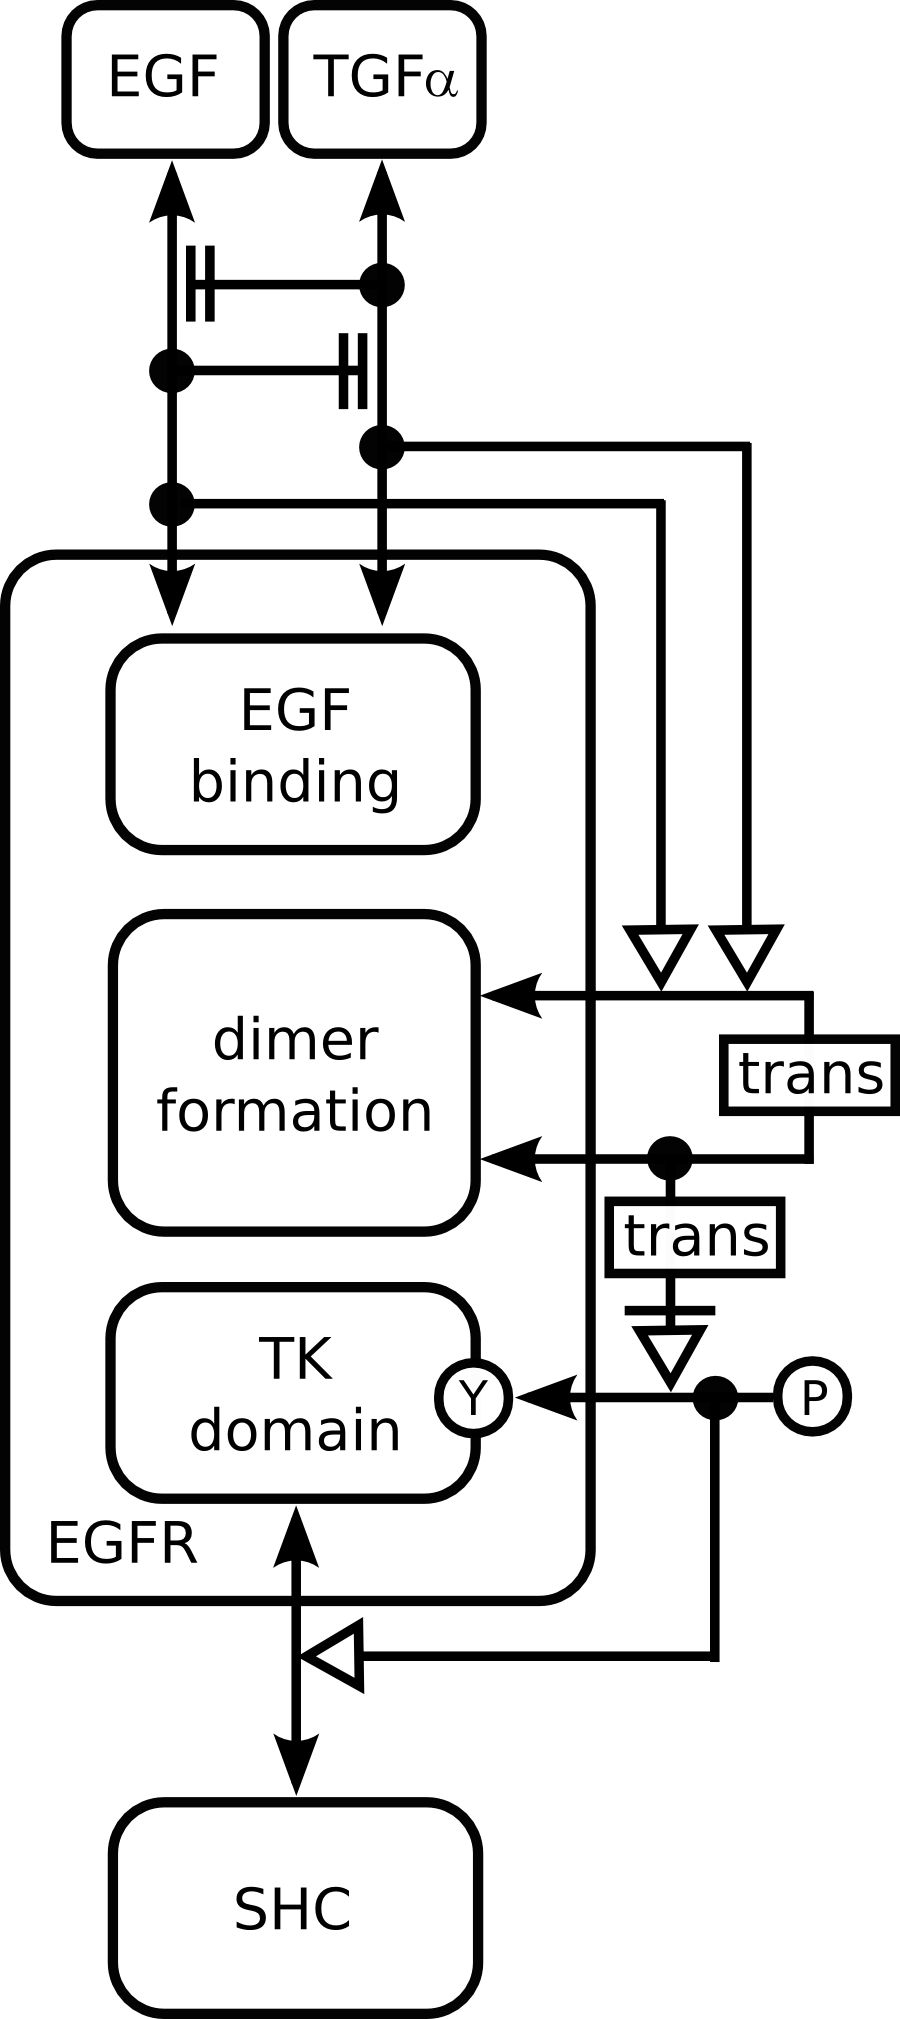
\includegraphics{figs/pngs/example_EGFR.png}
\caption{Binding of EGF on EGF receptor stimulates the dimerization of the latter, that then autophosphorylate. This phosphorylation increases the binding of SHC to the receptor. The figure is drawn using the SBGN Entity Relationship language.}
\label{fig:EGFR}
\end{center}
\end{figure}

\begin{example}
<?xml version="1.0" encoding="UTF-8"?>
<sbml xmlns="http://www.sbml.org/sbml/level3/version1/core" level="3" version="1"
      xmlns:multi="http://www.sbml.org/sbml/level3/version1/multi/version1"
      multi:required="true">

  <model name="EGF receptor">

<!-- -------------------------------------------------------------------------------- -->
<!-- Three compartments are defined, to contain the different species taking part     -->
<!-- to the EGFR reactions                                                            -->
<!-- -------------------------------------------------------------------------------- -->

    <listOfCompartments>
      <compartment id="extracellular" constant="true" spatialDimension="3" size="1" />
      <compartment id="membrane" constant="true" spatialDimension="2" size="1" />
      <compartment id="intracellular" constant="true" spatialDimension="3" size="1" />
    </listOfCompartments>

<!-- -------------------------------------------------------------------------------- -->
<!-- We need to define seven species types to be able to describe all the reactions.  -->
<!-- -------------------------------------------------------------------------------- -->

    <multi:listOfSpeciesTypes>
      <multi:speciesType multi:id="st_EGF" multi:name="EGF" multi:bindingSite="yes">
      <multi:speciesType multi:id="st_TGF" multi:name="TGF" multi:bindingSite="yes">
      <multi:speciesType multi:id="st_EGFBS" multi:name="EGF binding site" multi:bindingSite="true" />
      <multi:speciesType multi:id="st_dimer" multi:name="dimerisation domain" multi:bindingSite="true" />
      <multi:speciesType multi:id="st_signal" multi:name="signalling domain" multi:bindingSite="true">
         <multi:listOfStateFeatures>
           <multi:stateFeature multi:id="Y" multi:name="tyrosine">
             <multi:listOfPossibleValues>
               <multi:possibleValue multi:id="P" name="phosphorylated" />
               <multi:possibleValue multi:id="NP" name="non-phosphorylated" />
             </multi:listOfPossibleValues>
           </multi:stateFeature>
         </multi:listOfStateFeatures>
      </multi:speciesType>
      <multi:speciesType multi:id="st_EGFR" multi:name="EGFR" multi:bindingSite="no">   
      <multi:speciesType multi:id="st_SHC" multi:name="SHC" multi:bindingSite="yes">
    </multi:listOfSpeciesTypes>

<!-- -------------------------------------------------------------------------------- -->
<!-- Selectors are used to describe topologies and connectivities used in the model.  -->
<!-- -------------------------------------------------------------------------------- -->

    <multi:listOfSelectors>
\end{example}


\includegraphics{figs/pngs/sel_freeEGF.png}

\begin{example}
<!-- -------------------------------------------------------------------------------- -->
<!-- Description of free EGF, not bound                                               -->
<!-- -------------------------------------------------------------------------------- -->

      <multi:selector multi:id="sel_freeEGF">
        <multi:listOfSpeciesTypeStates>
          <multi:speciesTypeState multi:id="sts_EGF" multi:speciesType="st_EGF" 
                                  multi:minOccur="1" multi:maxOccur="1" />
        </multi:listOfSpeciesTypeStates>
        <multi:listOfUnboundBindingSites>
          <multi:bindingSiteReference multi:speciesTypeState="sts_EGF" />
        </multi:listOfUnboundBindingSites>
      </multi:selector>
\end{example}


\includegraphics{figs/pngs/sel_boundEGF.png}

\begin{example}
<!-- -------------------------------------------------------------------------------- -->
<!-- Description of EGF bound (to EGFR but this is not precised).                     -->
<!-- -------------------------------------------------------------------------------- -->

      <multi:selector multi:id="sel_boundEGF">
        <multi:listOfSpeciesTypeStates>
          <multi:speciesTypeState multi:id="sts_EGF" multi:speciesType="st_EGF" 
                                   multi:minOccur="1" multi:maxOccur="1" />
        </multi:listOfSpeciesTypeStates>
        <multi:listOfBonds>
          <multi:bond occurence="required">
            <multi:bindingSiteReference multi:speciesTypeState="sts_EGF" />
          </multi:bond>
        </multi:listOfBonds>
      </multi:selector>
\end{example}


\includegraphics{figs/pngs/sel_freeTGF.png}

\begin{example}
<!-- -------------------------------------------------------------------------------- -->
<!-- Description of free TGF, not bound                                               -->
<!-- -------------------------------------------------------------------------------- -->

      <multi:selector multi:id="sel_freeTGF">
        <multi:listOfSpeciesTypeStates>
          <multi:speciesTypeState multi:id="sts_TGF" multi:speciesType="st_TGF" 
                                   multi:minOccur="1" multi:maxOccur="1" />
        </multi:listOfSpeciesTypeStates>
        <multi:listOfUnboundBindingSites>
          <multi:bindingSiteReference multi:speciesTypeState="sts_TGF" />
        </multi:listOfUnboundBindingSites>
      </multi:selector>
\end{example}


\includegraphics{figs/pngs/sel_boundTGF.png}

\begin{example}
<!-- -------------------------------------------------------------------------------- -->
<!-- Description of TGF bound (to EGFR but this is not precised)                      -->
<!-- -------------------------------------------------------------------------------- -->

      <multi:selector multi:id="sel_boundTGF">
        <multi:listOfSpeciesTypeStates>
          <multi:speciesTypeState multi:id="sts_TGF" multi:speciesType="st_TGF" 
                                   multi:minOccur="1" multi:maxOccur="1" />
        </multi:listOfSpeciesTypeStates>
        <multi:listOfBonds>
          <multi:bond occurence="required">
            <multi:bindingSiteReference multi:speciesTypeState="sts_TGF" />
          </multi:bond>
        </multi:listOfBonds>
      </multi:selector>
\end{example}

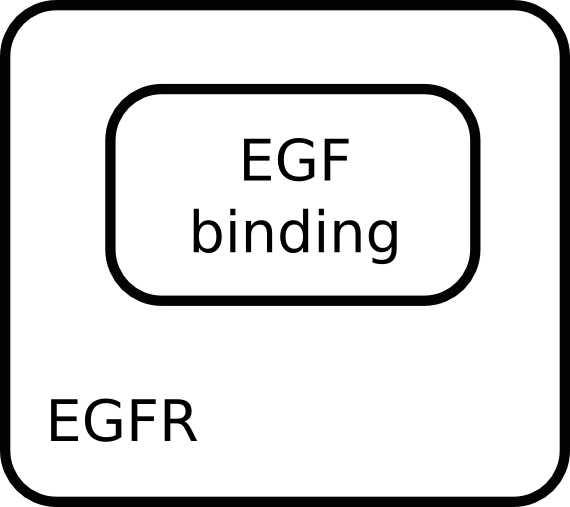
\includegraphics{figs/pngs/sel_freeEGFBS.png}

\begin{example}
<!-- -------------------------------------------------------------------------------- -->
<!-- Description of free EGF binding site, not bound to EGF or TGF.                   -->
<!-- -------------------------------------------------------------------------------- -->

      <multi:selector multi:id="sel_freeEGFBS">
        <multi:listOfSpeciesTypeStates>
          <multi:speciesTypeState multi:id="sts_EGFBS" multi:speciesType="st_EGFBS" 
                                   multi:minOccur="1" multi:maxOccur="1" />
          <multi:speciesTypeState multi:id="sts_EGFR" multi:speciesType="st_EGFR" 
                                   multi:minOccur="1" multi:maxOccur="1" >
            <multi:listOfContainedSpeciesTypes>
              <multi:containedSpeciesType multi:speciesTypeState="sts_EGFBS" /> 
            </multi:listOfContainedSpeciesType>            
          </multi:speciesTypeState>
        </multi:listOfSpeciesTypeStates>
        <multi:listOfUnboundBindingSites>
          <multi:bindingSiteReference multi:speciesTypeState="sts_EGFBS" />
        </multi:listOfUnboundBindingSites>
      </multi:selector>
\end{example}

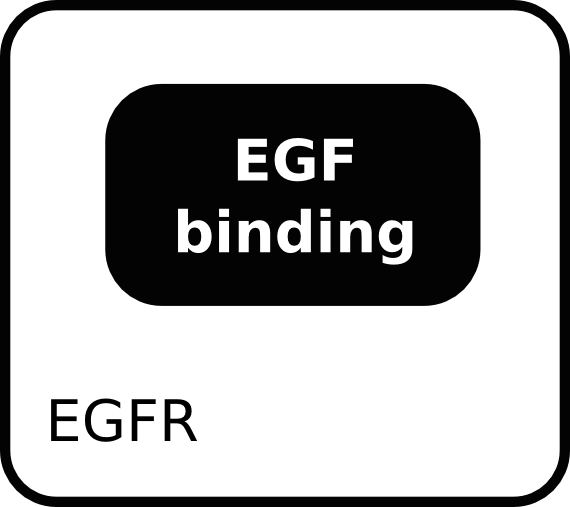
\includegraphics{figs/pngs/sel_boundEGFBS.png}

\begin{example}
<!-- -------------------------------------------------------------------------------- -->
<!-- Description of EGF binding site bound (either to EGF or TGF but this is not      -->
<!-- precised. Another approach would have been to create two selectors, describing   -->
<!-- EGFR bound to EGF and EGFR bound to TGF, and combine them at the level of the    -->
<!-- species.                                                                         -->
<!-- -------------------------------------------------------------------------------- -->

      <multi:selector multi:id="sel_boundEGFBS">
        <multi:listOfSpeciesTypeStates>
          <multi:speciesTypeState multi:id="sts_EGFBS" multi:speciesType="st_EGFBS" 
                                   multi:minOccur="1" multi:maxOccur="1" />
          <multi:speciesTypeState multi:id="sts_EGFR" multi:speciesType="st_EGFR" 
                                   multi:minOccur="1" multi:maxOccur="1" >
            <multi:listOfContainedSpeciesTypes>
              <multi:containedSpeciesType multi:speciesTypeState="sts_EGFBS" /> 
            </multi:listOfContainedSpeciesType>          
          </multi:speciesTypeState>
        </multi:listOfSpeciesTypeStates>
        <multi:listOfBonds>
          <multi:bond occurence="required">
            <multi:bindingSiteReference multi:speciesTypeState="sts_EGFBS" />
          </multi:bond>
        </multi:listOfBonds>
      </multi:selector>
\end{example}

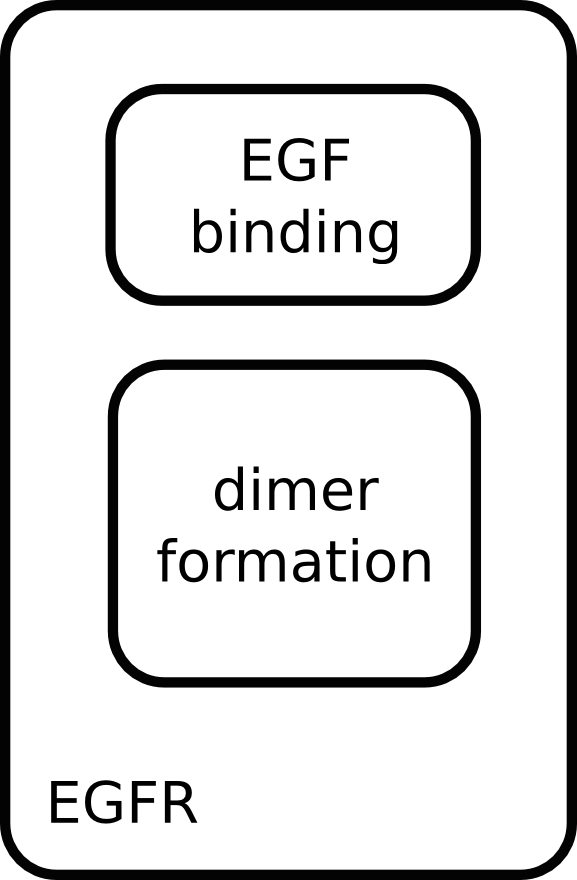
\includegraphics{figs/pngs/sel_freeDimerNoligand.png}

\begin{example}
<!-- -------------------------------------------------------------------------------- -->
<!-- Description of free EGFR dimerisation domain, not bound to another one, but in   --> 
<!-- receptors that are not bound to EGF or TGF.                                      -->
<!-- -------------------------------------------------------------------------------- -->

      <multi:selector multi:id="sel_freeDimerNoligand">
        <multi:listOfSpeciesTypeStates>
          <multi:speciesTypeState multi:id="sts_EGFBS" multi:speciesType="st_EGFBS" 
                                  multi:minOccur="1" multi:maxOccur="1" />
          <multi:speciesTypeState multi:id="sts_dimer" multi:speciesType="st_dimer" 
                                  multi:minOccur="1" multi:maxOccur="1" />
          </multi:speciesTypeState>
          <multi:speciesTypeState multi:id="sts_EGFR" multi:speciesType="st_EGFR" 
                                  multi:minOccur="1" multi:maxOccur="1" >
            <multi:listOfContainedSpeciesTypes>
              <multi:containedSpeciesType multi:speciesTypeState="sts_EGFBS" /> 
              <multi:containedSpeciesType multi:speciesTypeState="sts_dimer" /> 
            </multi:listOfContainedSpeciesTypes>            
          </multi:speciesTypeState>
        </multi:listOfSpeciesTypeStates>
        <multi:listOfUnboundBindingSites>
          <multi:bindingSiteReference multi:speciesTypeState="sts_dimer" />
          <multi:bindingSiteReference multi:speciesTypeState="sts_EGFBS" />
        </multi:listOfUnboundBindingSites>
      </multi:selector>
\end{example}

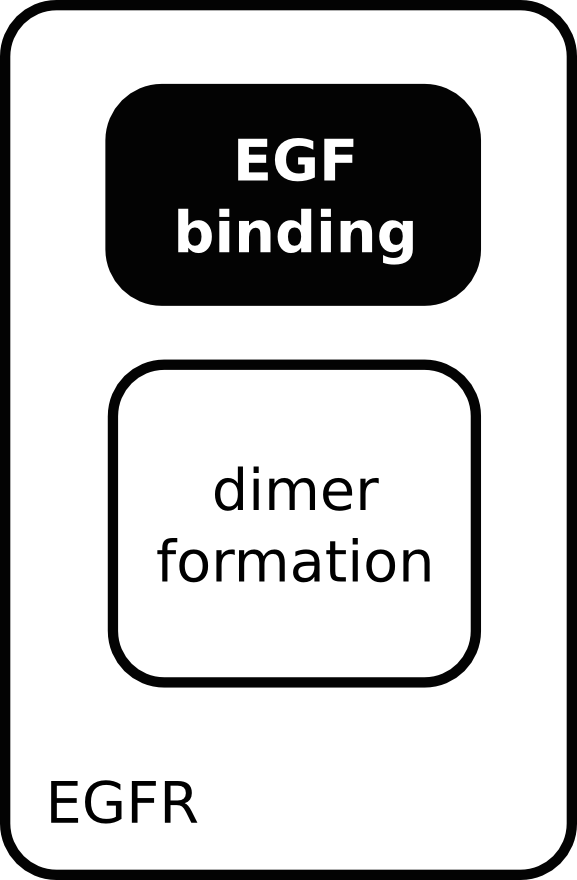
\includegraphics{figs/pngs/sel_freeDimerLigand.png}

\begin{example}
<!-- -------------------------------------------------------------------------------- -->
<!-- Description of free EGFR dimerisation domain, not bound to another one, but in   --> 
<!-- receptors that are bound to EGF or TGF.                                          -->
<!-- -------------------------------------------------------------------------------- -->

      <multi:selector multi:id="sel_freeDimerLigand">
        <multi:listOfSpeciesTypeStates>
          <multi:speciesTypeState multi:id="sts_EGFBS" multi:speciesType="st_EGFBS" 
                                   multi:minOccur="1" multi:maxOccur="1" />
          <multi:speciesTypeState multi:id="sts_dimer" multi:speciesType="st_dimer" 
                                   multi:minOccur="1" multi:maxOccur="1" />
          </multi:speciesTypeState>
          <multi:speciesTypeState multi:id="sts_EGFR" multi:speciesType="st_EGFR" 
                                   multi:minOccur="1" multi:maxOccur="1" >
            <multi:listOfContainedSpeciesTypes>
              <multi:containedSpeciesType multi:speciesTypeState="sts_EGFBS" /> 
              <multi:containedSpeciesType multi:speciesTypeState="sts_dimer" /> 
            </multi:listOfContainedSpeciesTypes>            
          </multi:speciesTypeState>
        </multi:listOfSpeciesTypeStates>
        <multi:listOfBonds>
          <multi:bond occurence="required">
            <multi:bindingSiteReference multi:speciesTypeState="sts_EGFBS" />
          </multi:bond>
        </multi:listOfBonds>
        <multi:listOfUnboundBindingSites>
          <multi:bindingSiteReference multi:speciesTypeState="sts_dimer" />
        </multi:listOfUnboundBindingSites>
      </multi:selector>
\end{example}

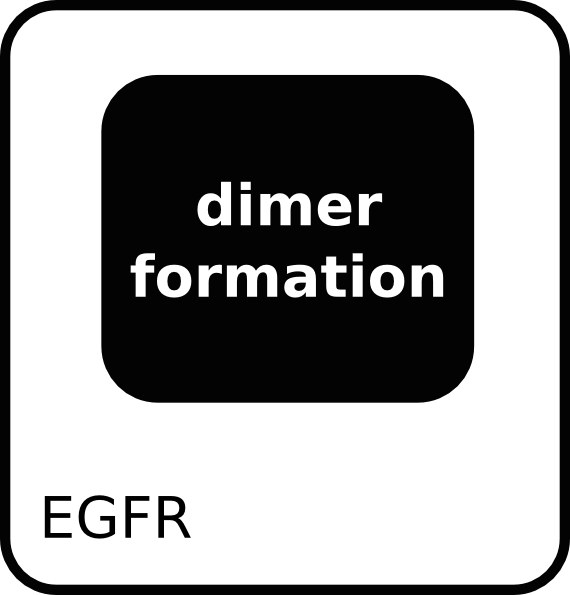
\includegraphics{figs/pngs/sel_boundDimer.png}

\begin{example}
<!-- -------------------------------------------------------------------------------- -->
<!-- Description of EGFR dimerisation domain bound (to another one but this is not    -->
<!-- described here)                                                                  -->
<!-- -------------------------------------------------------------------------------- -->

      <multi:selector multi:id="sel_boundDimer">
        <multi:listOfSpeciesTypeStates>
          <multi:speciesTypeState multi:id="sts_dimer" multi:speciesType="st_dimer" 
                                   multi:minOccur="1" multi:maxOccur="1" />
          <multi:speciesTypeState multi:id="sts_EGFR" multi:speciesType="st_EGFR" 
                                   multi:minOccur="1" multi:maxOccur="1" >
            <multi:listOfContainedSpeciesTypes>
              <multi:containedSpeciesType multi:speciesTypeState="sts_dimer" /> 
            </multi:listOfContainedSpeciesTypes>            
          </multi:speciesTypeState>
        </multi:listOfSpeciesTypeStates>
        <multi:listOfBonds>
          <multi:bond occurence="required">
            <multi:bindingSiteReference multi:speciesTypeState="sts_dimer" />
          </multi:bond>
        </multi:listOfBonds>
      </multi:selector>
\end{example}

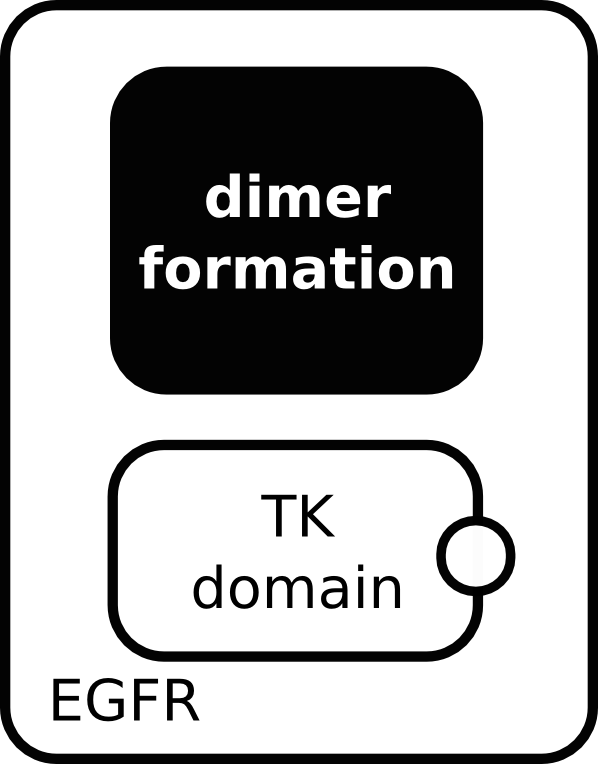
\includegraphics{figs/pngs/sel_EGFRDimerNonPhos.png}

\begin{example}
<!-- -------------------------------------------------------------------------------- -->
<!-- Description of EGFR dimerised with one signalling domain non-phosphorylated      -->
<!-- -------------------------------------------------------------------------------- -->

      <multi:selector multi:id="sel_EGFRDimerNonPhos">
        <multi:listOfSpeciesTypeStates>
          <multi:speciesTypeState multi:id="sts_dimer" multi:speciesType="st_dimer" 
                                   multi:minOccur="1" multi:maxOccur="1" />
          <multi:speciesTypeState multi:id="sts_signal" multi:speciesType="st_signal" 
                                   multi:minOccur="1" multi:maxOccur="1">
            <multi:listOfStateFeatureInstances>
              <multi:stateFeatureInstance multi:stateFeature="Y">
                <multi:listOfStateFeatureValues>
                  <multi:stateFeatureValue multi:possibleValue="NP" />
                </multi:listOfStateFeatureValues>
              </multi:stateFeatureInstance>
            </multi:listOfStateFeatureInstances>
          </multi:speciesTypeState>
          <multi:speciesTypeState multi:id="sts_EGFR" multi:speciesType="st_EGFR" 
                                   multi:minOccur="1" multi:maxOccur="1" >
            <multi:listOfContainedSpeciesTypes>
              <multi:containedSpeciesType multi:speciesTypeState="sts_dimer" /> 
              <multi:containedSpeciesType multi:speciesTypeState="sts_signal" /> 
            </multi:listOfContainedSpeciesTypes>            
          </multi:speciesTypeState>
        </multi:listOfSpeciesTypeStates>
        <multi:listOfBonds>
          <multi:bond occurence="required">
            <multi:bindingSiteReference multi:speciesTypeState="sts_dimer" />
          </multi:bond>
        </multi:listOfBonds>
      </multi:selector>
\end{example}

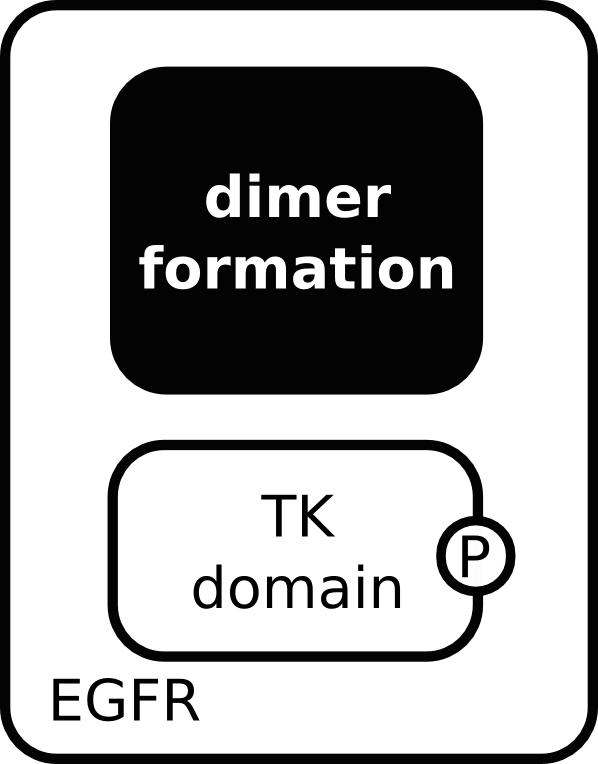
\includegraphics{figs/pngs/sel_EGFRDimerPhos.png}

\begin{example}
<!-- -------------------------------------------------------------------------------- -->
<!-- Description of EGFR dimerised with one signalling domain phosphorylated          --> 
<!-- -------------------------------------------------------------------------------- -->

      <multi:selector multi:id="sel_EGFRDimerPhos">
        <multi:listOfSpeciesTypeStates>
          <multi:speciesTypeState multi:id="sts_dimer" multi:speciesType="st_dimer" 
                                   multi:minOccur="1" multi:maxOccur="1" />
          <multi:speciesTypeState multi:id="sts_signal" multi:speciesType="st_signal" 
                                   multi:minOccur="1" multi:maxOccur="1">
            <multi:listOfStateFeatureInstances>
              <multi:stateFeatureInstance multi:stateFeature="Y">
                <multi:listOfStateFeatureValues>
                  <multi:stateFeatureValue multi:possibleValue="P" />
                </multi:listOfStateFeatureValues>
              </multi:stateFeatureInstance>
            </multi:listOfStateFeatureInstances>
          </multi:speciesTypeState>
          <multi:speciesTypeState multi:id="sts_EGFR" multi:speciesType="st_EGFR" 
                                   multi:minOccur="1" multi:maxOccur="1" >
            <multi:listOfContainedSpeciesTypes>
              <multi:containedSpeciesType multi:speciesTypeState="sts_dimer" /> 
              <multi:containedSpeciesType multi:speciesTypeState="sts_signal" /> 
            </multi:listOfContainedSpeciesTypes>            
          </multi:speciesTypeState>
        </multi:listOfSpeciesTypeStates>
        <multi:listOfBonds>
          <multi:bond occurence="required">
            <multi:bindingSiteReference multi:speciesTypeState="sts_dimer" />
          </multi:bond>
        </multi:listOfBonds>
      </multi:selector>
\end{example}


\includegraphics{figs/pngs/sel_freeSHC.png}

\begin{example}
<!-- -------------------------------------------------------------------------------- -->
<!-- Description of free SHC, not bound to EGFR.                                      -->
<!-- -------------------------------------------------------------------------------- -->

      <multi:selector multi:id="sel_freeSHC">
        <multi:listOfSpeciesTypeStates>
          <multi:speciesTypeState multi:id="sts_SHC" multi:speciesType="st_SHC" 
                                   multi:minOccur="1" multi:maxOccur="1" />
        </multi:listOfSpeciesTypeStates>
        <multi:listOfUnboundBindingSites>
          <multi:bindingSiteReference multi:speciesTypeState="sts_SHC" />
        </multi:listOfUnboundBindingSites>
      </multi:selector>
\end{example}


\includegraphics{figs/pngs/sel_SHC_Signal.png}

\begin{example}
<!-- -------------------------------------------------------------------------------- -->
<!-- Description of SHC bound to EGFR signalling domain                               -->
<!-- -------------------------------------------------------------------------------- -->

      <multi:selector multi:id="sel_SHC_Signal">
        <multi:listOfSpeciesTypeStates>
          <multi:speciesTypeState multi:id="sts_SHC" multi:speciesType="st_SHC" 
                                   multi:minOccur="1" multi:maxOccur="1" />
          <multi:speciesTypeState multi:id="sts_signal" multi:speciesType="st_signal" 
                                   multi:minOccur="1" multi:maxOccur="1" />
          </multi:speciesTypeState>
        </multi:listOfSpeciesTypeStates>
        <multi:listOfBonds>
          <multi:bond occurence="required">
            <multi:bindingSiteReference multi:speciesTypeState="sts_SHC" />
            <multi:bindingSiteReference multi:speciesTypeState="sts_signal" />
          </multi:bond>
        </multi:listOfBonds>
      </multi:selector>
\end{example}

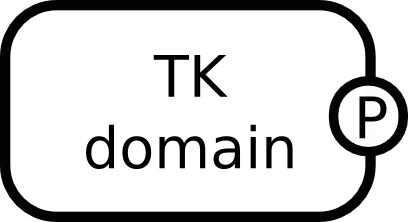
\includegraphics{figs/pngs/sel_freeEGFRPhos.png}

\begin{example}
<!-- -------------------------------------------------------------------------------- -->
<!-- EGFR signalling domain phosphorylated and not bound to SHC                       --> 
<!-- -------------------------------------------------------------------------------- -->

      <multi:selector multi:id="sel_freeEGFRPhos">
        <multi:listOfSpeciesTypeStates>
          <multi:speciesTypeState multi:id="sts_signal" multi:speciesType="st_signal" 
                                   multi:minOccur="1" multi:maxOccur="1">
            <multi:listOfStateFeatureInstances>
              <multi:stateFeatureInstance multi:stateFeature="Y">
                <multi:listOfStateFeatureValues>
                  <multi:stateFeatureValue multi:possibleValue="P" />
                </multi:listOfStateFeatureValues>
              </multi:stateFeatureInstance>
            </multi:listOfStateFeatureInstances>
          </multi:speciesTypeState>
        </multi:listOfSpeciesTypeStates>
        <multi:listOfUnboundBindingSites>
          <multi:bindingSiteReference multi:speciesTypeState="sts_signal" />
        </multi:listOfUnboundBindingSites>
      </multi:selector>
\end{example}

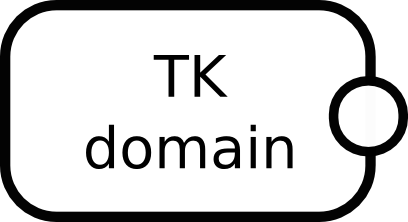
\includegraphics{figs/pngs/sel_freeEGFRNonPhos.png}

\begin{example}
<!-- -------------------------------------------------------------------------------- -->
<!-- EGFR signalling domain non-phosphorylated and not bound to SHC                   --> 
<!-- -------------------------------------------------------------------------------- -->

      <multi:selector multi:id="sel_freeEGFRNonPhos">
        <multi:listOfSpeciesTypeStates>
          <multi:speciesTypeState multi:id="sts_signal" multi:speciesType="st_signal" 
                                   multi:minOccur="1" multi:maxOccur="1">
            <multi:listOfStateFeatureInstances>
              <multi:stateFeatureInstance multi:stateFeature="Y">
                <multi:listOfStateFeatureValues>
                  <multi:stateFeatureValue multi:possibleValue="NP" />
                </multi:listOfStateFeatureValues>
              </multi:stateFeatureInstance>
            </multi:listOfStateFeatureInstances>
          </multi:speciesTypeState>
        </multi:listOfSpeciesTypeStates>
        <multi:listOfUnboundBindingSites>
          <multi:bindingSiteReference multi:speciesTypeState="sts_signal" />
        </multi:listOfUnboundBindingSites>
      </multi:selector>

   </multi:listOfSelectors>

<!-- -------------------------------------------------------------------------------- -->
<!-- Six species describe the entities actually present in the simulations.           -->
<!-- -------------------------------------------------------------------------------- -->

    <listOfSpecies>

<!-- -------------------------------------------------------------------------------- -->
<!-- EGF, can be free or bound                                                        -->
<!-- -------------------------------------------------------------------------------- -->

      <species id="EGF" compartment="extracellular" multi:speciesType="st_EGF"
               boundaryCondition="false" hasOnlySubstanceUnit="false" 
               constant="false" initialAmount="500" >
        <multi:listOfSpeciesTypeInstances>
          <multi:SpeciesTypeInstance multi:id="freeEGF" multi:initialAmount="500">
            <multi:listOfSelectorReferences>
              <multi:selectorReference multi:selector="sel_freeEGF" multi:negation="false"/>
            </multi:listOfSelectorReferences>
          </multi:speciesTypeInstance>
          <multi:SpeciesTypeInstance multi:id="boundEGF">
            <multi:listOfSelectorReferences>
              <multi:selectorReference multi:selector="sel_boundEGF" multi:negation="false"/>
            </multi:listOfSelectorReferences>
        </multi:listOfSpeciesTypeInstances>
      </species>

<!-- -------------------------------------------------------------------------------- -->
<!-- TGF, can be free or bound                                                        -->
<!-- -------------------------------------------------------------------------------- -->

     <species id="TGF" compartment="extracellular" multi:speciesType="st_TGF"
               boundaryCondition="false" hasOnlySubstanceUnit="false" 
               constant="false" initialAmount="500" >
        <multi:listOfSpeciesTypeInstances>
          <multi:SpeciesTypeInstance multi:id="freeTGF" multi:initialAmount="500">
            <multi:listOfSelectorReferences>
              <multi:selectorReference multi:selector="sel_freeTGF" multi:negation="false"/>
            </multi:listOfSelectorReferences>
          </multi:speciesTypeInstance>
          <multi:SpeciesTypeInstance multi:id="boundTGF">
            <multi:listOfSelectorReferences>
              <multi:selectorReference multi:selector="sel_boundTGF" multi:negation="false"/>
            </multi:listOfSelectorReferences>
        </multi:listOfSpeciesTypeInstances>
      </species>

<!-- -------------------------------------------------------------------------------- -->
<!-- EGF binding site, can be free or bound                                           -->
<!-- -------------------------------------------------------------------------------- -->

      <species id="EGFBS" compartment="extracellular" multi:speciesType="st_EGFBS"
               boundaryCondition="false" hasOnlySubstanceUnit="false" 
               constant="false" initialAmount="50" >
        <multi:listOfSpeciesTypeInstances>
          <multi:SpeciesTypeInstance multi:id="freeEGFBS" multi:initialAmount="50">
            <multi:listOfSelectorReferences>
              <multi:selectorReference multi:selector="sel_freeEGFBS" multi:negation="false"/>
            </multi:listOfSelectorReferences>
          </multi:speciesTypeInstance>
          <multi:SpeciesTypeInstance multi:id="boundEGFBS">
            <multi:listOfSelectorReferences>
              <multi:selectorReference multi:selector="sel_boundEGFBS" multi:negation="false"/>
            </multi:listOfSelectorReferences>
        </multi:listOfSpeciesTypeInstances>
      </species>

<!-- -------------------------------------------------------------------------------- -->
<!-- EGF dimerisation domain, can be free or bound                                    -->
<!-- -------------------------------------------------------------------------------- -->

      <species id="dimer" compartment="membrane" multi:speciesType="st_dimer"
               boundaryCondition="false" hasOnlySubstanceUnit="false" 
               constant="false" initialAmount="50" >
        <multi:listOfSpeciesTypeInstances>
          <multi:SpeciesTypeInstance multi:id="freeDimerNoligand" multi:initialAmount="50">
            <multi:listOfSelectorReferences>
              <multi:selectorReference multi:selector="sel_freeDimerNoligand" multi:negation="false"/>
            </multi:listOfSelectorReferences>
          </multi:speciesTypeInstance>
          <multi:SpeciesTypeInstance multi:id="freeDimerLigand">
            <multi:listOfSelectorReferences>
              <multi:selectorReference multi:selector="sel_freeDimerNoligand" multi:negation="false"/>
            </multi:listOfSelectorReferences>
          <multi:SpeciesTypeInstance multi:id="boundDimer">
            <multi:listOfSelectorReferences>
              <multi:selectorReference multi:selector="sel_boundDimer" multi:negation="false"/>
            </multi:listOfSelectorReferences>
        </multi:listOfSpeciesTypeInstances>
      </species>

<!-- -------------------------------------------------------------------------------- -->
<!-- EGF signalling domain, can be phosphorylated or not, bound to SHC or not         -->
<!-- -------------------------------------------------------------------------------- -->

      <species id="signal" compartment="intracellular" multi:speciesType="st_signal"
               boundaryCondition="false" hasOnlySubstanceUnit="false" 
               constant="false" initialAmount="50" >
        <multi:listOfSpeciesTypeInstances>
          <multi:SpeciesTypeInstance multi:id="DimerNonPhosSignal" multi:initialAmount="50">
            <multi:listOfSelectorReferences>
              <multi:selectorReference multi:selector="sel_EGFRDimerNonPhos" multi:negation="false"/>
            </multi:listOfSelectorReferences>
          </multi:speciesTypeInstance>
          <multi:SpeciesTypeInstance multi:id="DimerPhosSignal">
            <multi:listOfSelectorReferences>
              <multi:selectorReference multi:selector="sel_EGFRDimerPhos" multi:negation="false"/>
            </multi:listOfSelectorReferences>
          </multi:speciesTypeInstance>
          <multi:SpeciesTypeInstance multi:id="freeNonPhosSignal">
            <multi:listOfSelectorReferences>
              <multi:selectorReference multi:selector="sel_freeEGFRNonPhos" multi:negation="false"/>
            </multi:listOfSelectorReferences>
          </multi:speciesTypeInstance>
          <multi:SpeciesTypeInstance multi:id="freePhosSignal">
            <multi:listOfSelectorReferences>
              <multi:selectorReference multi:selector="sel_freeEGFRPhos" multi:negation="false"/>
            </multi:listOfSelectorReferences>
          </multi:speciesTypeInstance>
           <multi:SpeciesTypeInstance multi:id="boundSignal">
            <multi:listOfSelectorReferences>
              <multi:selectorReference multi:selector="sel_SHC_Signal" multi:negation="false"/>
            </multi:listOfSelectorReferences>
          </multi:speciesTypeInstance>
       </multi:listOfSpeciesTypeInstances>
      </species>

<!-- -------------------------------------------------------------------------------- -->
<!-- SHC, can be free or bound                                                        -->
<!-- -------------------------------------------------------------------------------- -->

     <species id="SHC" compartment="extracellular" multi:speciesType="st_TGF"
               boundaryCondition="false" hasOnlySubstanceUnit="false" 
               constant="false" initialAmount="500" >
        <multi:listOfSpeciesTypeInstances>
          <multi:SpeciesTypeInstance multi:id="freeSHC" multi:initialAmount="500">
            <multi:listOfSelectorReferences>
              <multi:selectorReference multi:selector="sel_freeSHC" multi:negation="false"/>
            </multi:listOfSelectorReferences>
          </multi:speciesTypeInstance>
          <multi:SpeciesTypeInstance multi:id="boundSHC">
            <multi:listOfSelectorReferences>
              <multi:selectorReference multi:selector="sel_SHC_Signal" multi:negation="false"/>
            </multi:listOfSelectorReferences>
          </multi:speciesTypeInstance>
        </multi:listOfSpeciesTypeInstances>
      </species>


    </listOfSpecies>

<!-- -------------------------------------------------------------------------------- -->
<!-- 5 reactions are sufficient to describe the system                                -->
<!-- -------------------------------------------------------------------------------- -->

    <listOfReactions>
\end{example}

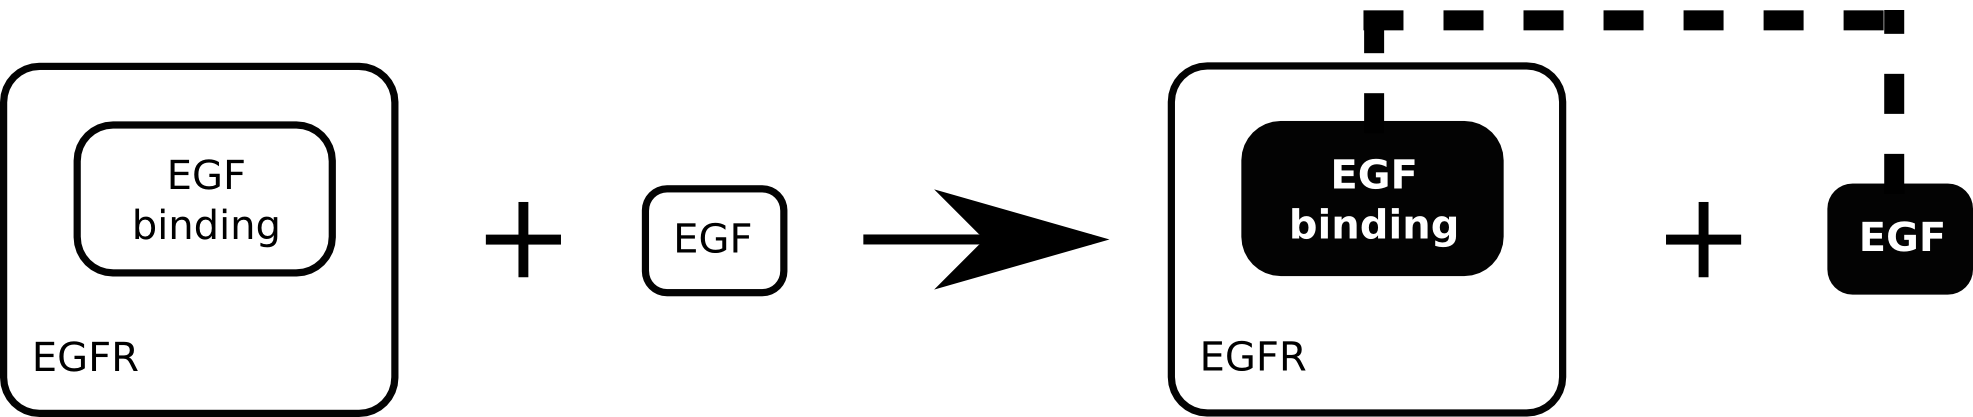
\includegraphics[scale=0.9]{figs/pngs/EGFbinding.png}

\begin{example}
<!-- -------------------------------------------------------------------------------- -->
<!-- Binding of EGF to EGF receptor.                                                  -->
<!-- -------------------------------------------------------------------------------- -->

       <reaction id="EGFbinding" reversible="false" fast="false"> 
        <listOfReactants>
          <speciesReference id="react_EGF" species="EGF" stoichiometry="1">
            <multi:listOfSpeciesRestriction>
              <multi:speciesRestriction multi:id="sr_freeEGF" 
                                        multi:speciesTypeInstance="freeEGF" />
            </multi:listOfSpeciesRestriction>
          </speciesReference>
          <speciesReference id="react_EGFBS" species="EGFBS" stoichiometry="1">
            <multi:listOfSpeciesRestriction>
              <multi:speciesRestriction multi:id="sr_freeEGFBS" 
                                        multi:speciesTypeInstance="freeEGFBS" />
            </multi:listOfSpeciesRestriction>
          </speciesReference>
        </listOfReactants>

<!-- -------------------------------------------------------------------------------- -->
<!-- In this binding reaction, and the following two, we represent the products       --> 
<!-- as separate components. See the binding of SHC on EGFR to see how we can also    --> 
<!-- represent complexes                                                              -->
<!-- -------------------------------------------------------------------------------- -->
 
        <listOfProducts>
          <multi:productSpeciesReference species="EGF" stoichiometry="1"
                                   correspondingReactant="react_EGF">
            <multi:listOfSpeciesRestriction>
              <multi:speciesRestriction multi:id="sr_boundEGF" 
                                        multi:speciesTypeInstance="boundEGF" />
            </multi:listOfSpeciesRestriction>
          </multi:productSpeciesReference>

<!-- -------------------------------------------------------------------------------- -->
<!-- Since only free EGF is involved in this reaction, and not TGF, it it sufficient  --> 
<!-- to describe EGFR bound, without precising what it is bound to.                   -->
<!-- -------------------------------------------------------------------------------- -->

          <multi:productSpeciesReference species="EGFBS" stoichiometry="1"
                                   correspondingReactant="react_EGFBS">
            <multi:listOfSpeciesRestriction>
              <multi:speciesRestriction multi:id="sr_boundEGFBS" 
                                        multi:speciesTypeInstance="boundEGFBS" />
            </multi:listOfSpeciesRestriction>
          </multi:productSpeciesReference>
        </listOfProducts>

        <multi:reactionRule multi:id="EGFbindingFreeSite">
          <multi:listOfConditions>
            <multi:speciesTypeRestrictionReference multi:speciesTypeRestriction="sr_freeEGF"/>
            <multi:speciesTypeRestrictionReference multi:speciesTypeRestriction="sr_freeEGFBS"/>
          </multi:listOfConditions>
          <multi:listOfResults>
            <multi:speciesTypeRestrictionReference multi:speciesTypeRestriction="sr_boundEGF"/>
            <multi:speciesTypeRestrictionReference multi:speciesTypeRestriction="sr_boundEGFBS"/>
          </multi:listOfResults>
            <kineticLaw>
              <math xmlns="http://www.w3.org/1998/Math/MathML" >
                <apply>
                  <times />
                  <ci> konegf </ci>
                  <ci> sr_freeEGF </ci>
                  <ci> sr_freeEGFBS </ci>
                  <ci> extracellular </ci>
                </apply>
              </math>
              <listOfLocalParameters>
                <localParameter id="konegf" value="10">
              </listOfLocalParameters>
            </kineticLaw>
          </multi:reactionRule>
      </reaction>
\end{example}

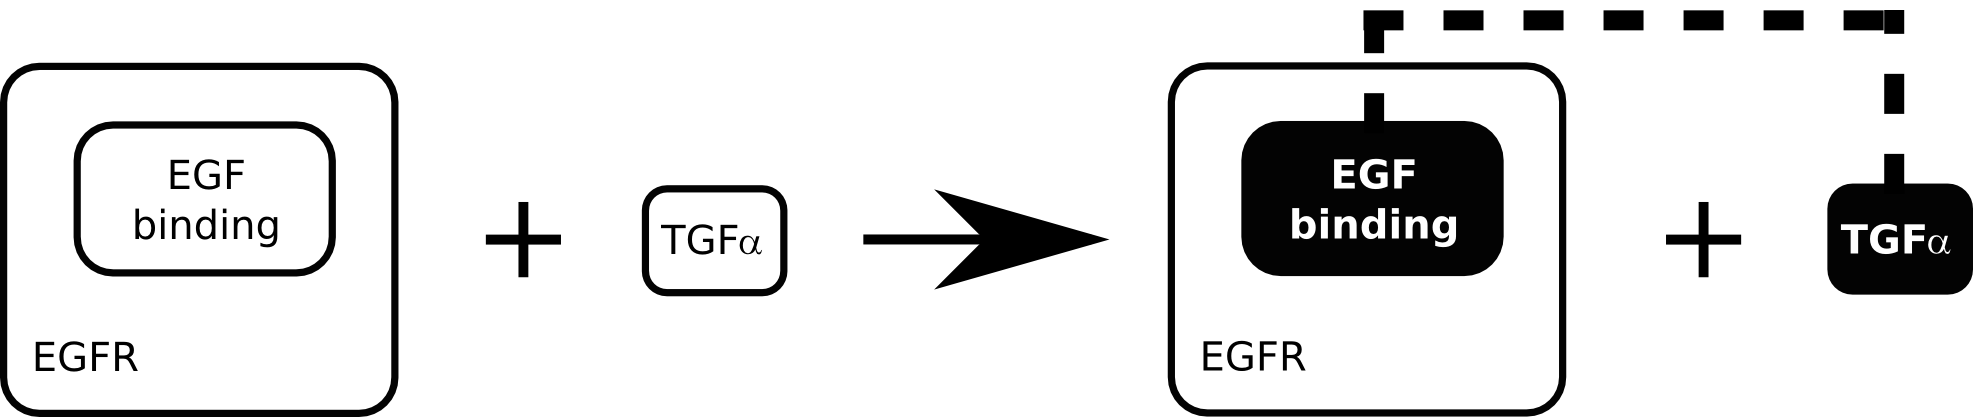
\includegraphics[scale=0.9]{figs/pngs/TGFbinding.png}

\begin{example}
<!-- -------------------------------------------------------------------------------- -->
<!-- Binding of TGF to EGF receptor.                                                  -->
<!-- -------------------------------------------------------------------------------- -->

       <reaction id="TGFbinding" reversible="false" fast="false"> 
        <listOfReactants>
          <speciesReference id="react_TGF" species="TGF" stoichiometry="1">
            <multi:listOfSpeciesRestriction>
              <multi:speciesRestriction multi:id="sr_freeTGF" 
                                        multi:speciesTypeInstance="freeTGF" />
            </multi:listOfSpeciesRestriction>
          </speciesReference>
          <speciesReference id="react_EGFBS" species="EGFBS" stoichiometry="1">
            <multi:listOfSpeciesRestriction>
              <multi:speciesRestriction multi:id="sr_freeEGFBS" 
                                        multi:speciesTypeInstance="freeEGFBS" />
            </multi:listOfSpeciesRestriction>
          </speciesReference>
        </listOfReactants>
        <listOfProducts>
          <multi:productSpeciesReference species="TGF" stoichiometry="1"
                                   correspondingReactant="react_TGF">
            <multi:listOfSpeciesRestriction>
              <multi:speciesRestriction multi:id="sr_boundTGF" 
                                        multi:speciesTypeInstance="boundTGF" />
            </multi:listOfSpeciesRestriction>
          </multi:productSpeciesReference>
          <multi:productSpeciesReference species="EGFBS" stoichiometry="1"
                                   correspondingReactant="react_EGFBS">
            <multi:listOfSpeciesRestriction>
              <multi:speciesRestriction multi:id="sr_boundEGFBS" 
                                        multi:speciesTypeInstance="boundEGFBS" />
            </multi:listOfSpeciesRestriction>
          </multi:productSpeciesReference>
        </listOfProducts>

        <multi:reactionRule multi:id="TGFbindingFreeSite">
          <multi:listOfConditions>
            <multi:speciesTypeRestrictionReference multi:speciesTypeRestriction="sr_freeTGF"/>
            <multi:speciesTypeRestrictionReference multi:speciesTypeRestriction="sr_freeEGFBS"/>
          </multi:listOfConditions>
          <multi:listOfResults>
            <multi:speciesTypeRestrictionReference multi:speciesTypeRestriction="sr_boundTGF"/>
            <multi:speciesTypeRestrictionReference multi:speciesTypeRestriction="sr_boundEGFBS"/>
          </multi:listOfResults>
            <kineticLaw>
              <math xmlns="http://www.w3.org/1998/Math/MathML" >
                <apply>
                  <times />
                  <ci> kontgf </ci>
                  <ci> sr_freeTGF </ci>
                  <ci> sr_freeEGFBS </ci>
                  <ci> extracellular </ci>
                </apply>
              </math>
              <listOfLocalParameters>
                <localParameter id="kontgf" value="5">
              </listOfLocalParameters>
            </kineticLaw>
          </multi:reactionRule>
        </reaction>
\end{example}

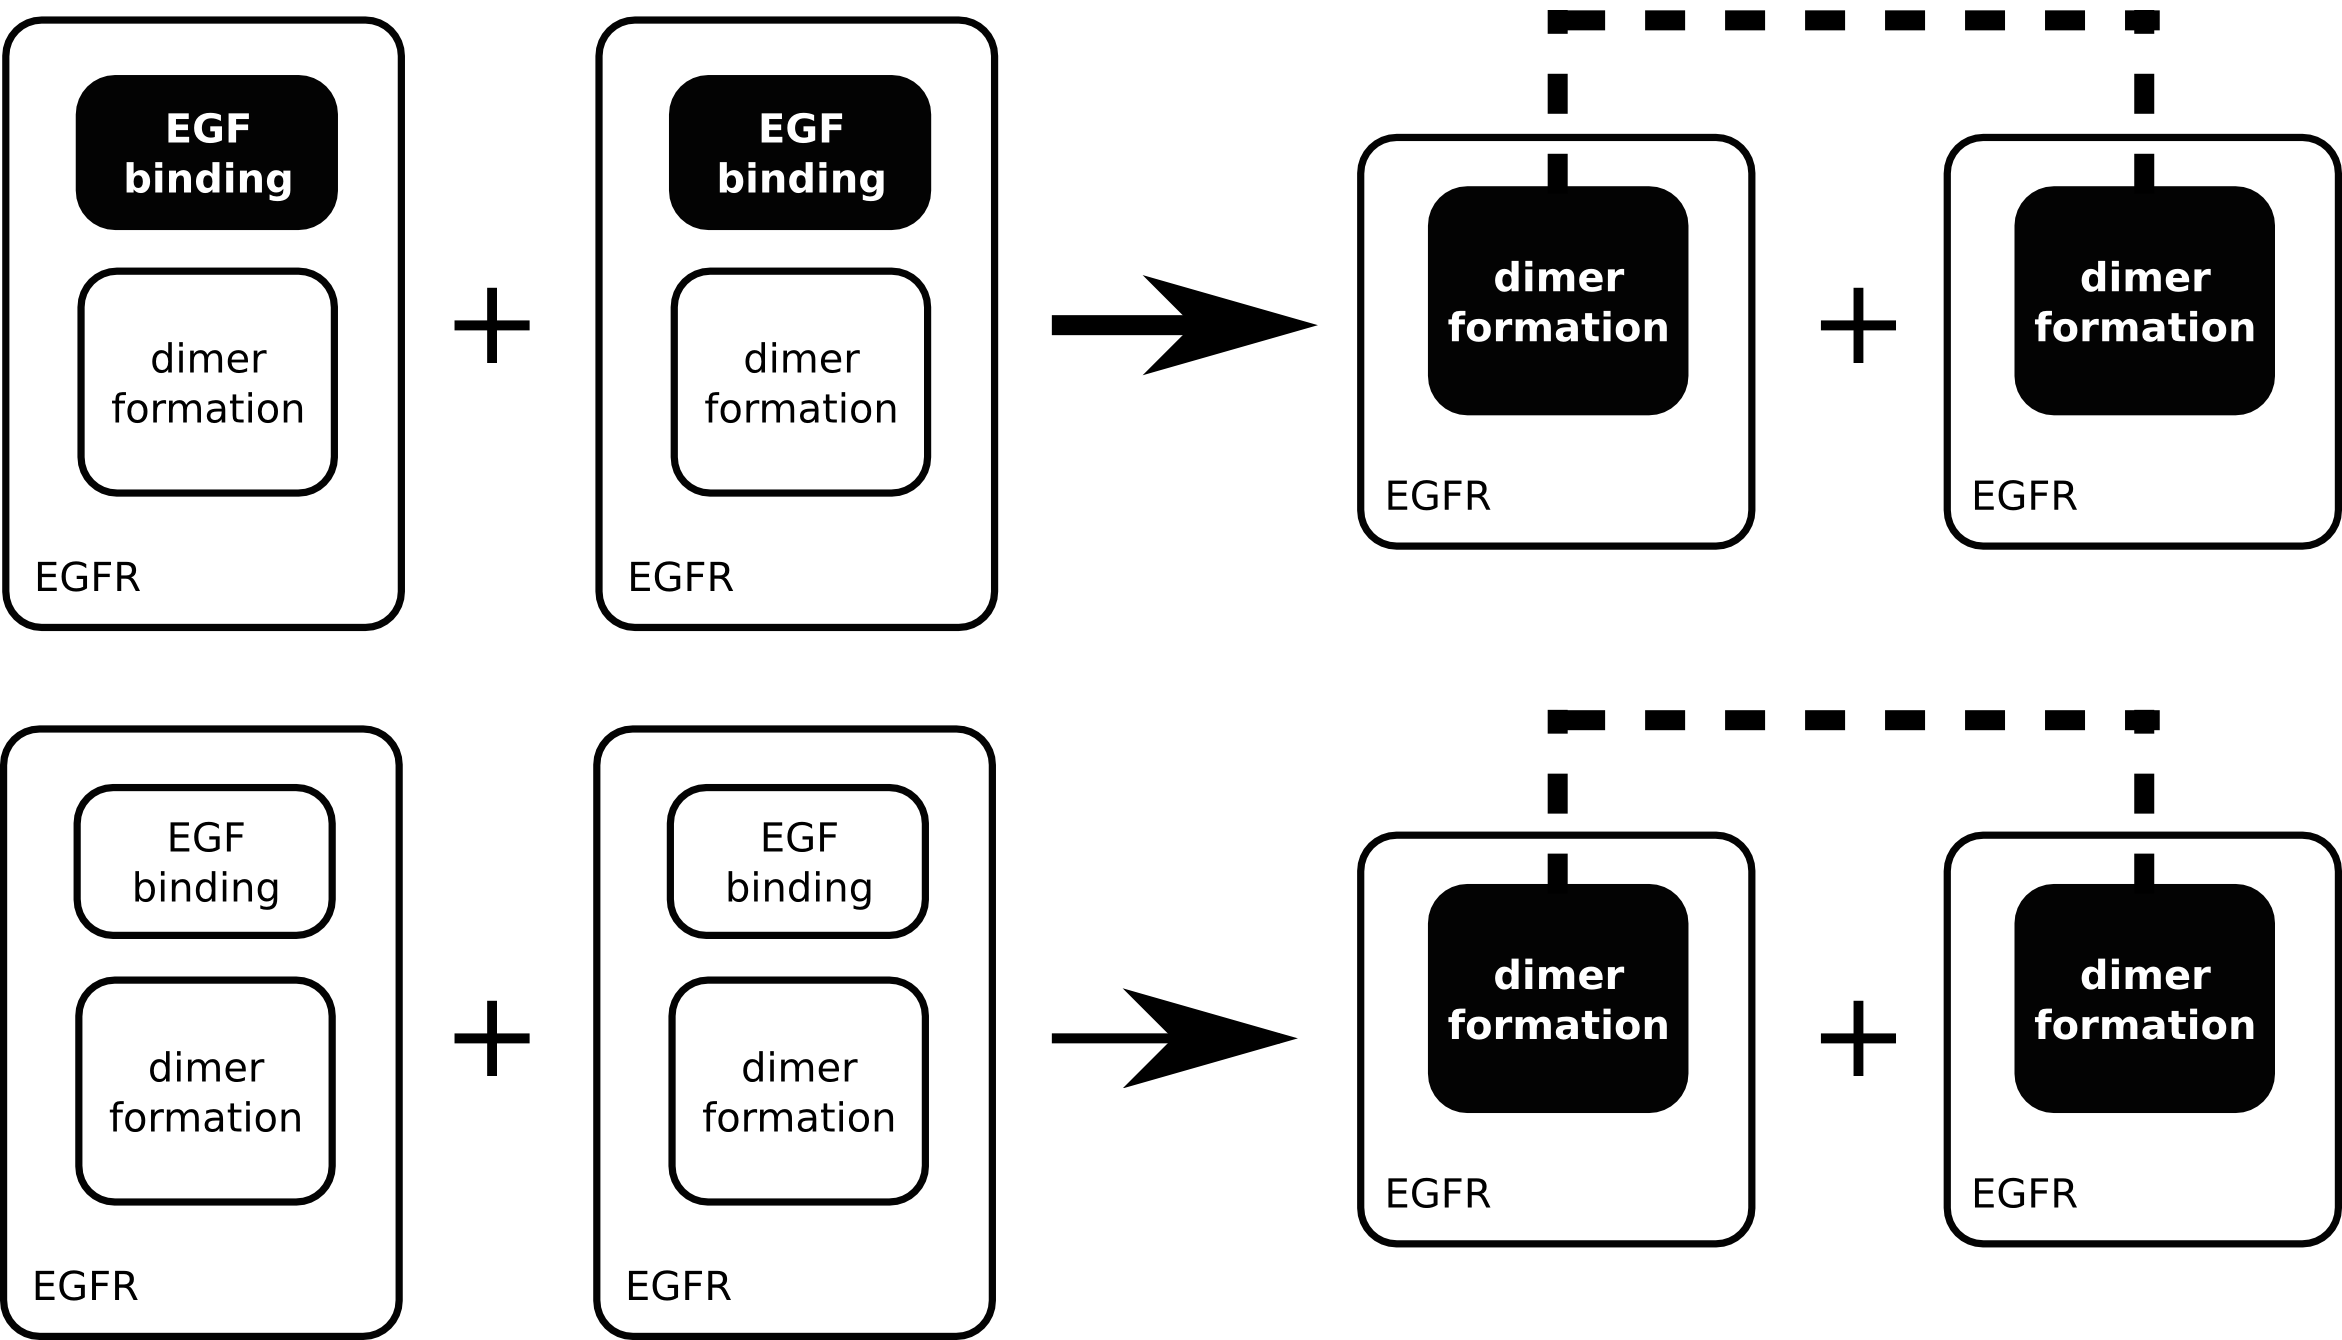
\includegraphics[scale=0.8]{figs/pngs/dimerisation.png}

\begin{example}
<!-- -------------------------------------------------------------------------------- -->
<!-- Dimerisation of receptor is stimulated when bound to a ligand                    -->
<!-- -------------------------------------------------------------------------------- -->

       <reaction id="dimerisation" reversible="false" fast="false"> 
        <listOfReactants>
          <speciesReference id="react_dimer1" species="dimer" stoichiometry="1">
            <multi:listOfSpeciesRestriction>
              <multi:speciesRestriction multi:id="sr_freeDimerNoligand1" 
                                        multi:speciesTypeInstance="freeDimerNoligand" />
              <multi:speciesRestriction multi:id="sr_freeDimerLigand1" 
                                        multi:speciesTypeInstance="freeDimerLigand" />
            </multi:listOfSpeciesRestriction>
          </speciesReference>
          <speciesReference id="react_dimer2" species="dimer" stoichiometry="1">
            <multi:listOfSpeciesRestriction>
              <multi:speciesRestriction multi:id="sr_freeDimerNoLigand2" 
                                        multi:speciesTypeInstance="freeDimerNoligand" />
              <multi:speciesRestriction multi:id="sr_freeDimerLigand2" 
                                        multi:speciesTypeInstance="freeDimerLigand" />
            </multi:listOfSpeciesRestriction>
          </speciesReference>
        </listOfReactants>
        <listOfProducts>
          <multi:productSpeciesReference species="dimer" stoichiometry="1"
                                   correspondingReactant="react_dimer1">
            <multi:listOfSpeciesRestriction>
              <multi:speciesRestriction multi:id="sr_boundDimer1" 
                                        multi:speciesTypeInstance="boundDimer />
            </multi:listOfSpeciesRestriction>
          </multi:productSpeciesReference>
          <multi:productSpeciesReference species="dimer" stoichiometry="1"
                                   correspondingReactant="react_dimer2">
            <multi:listOfSpeciesRestriction>
              <multi:speciesRestriction multi:id="sr_boundDimer2" 
                                        multi:speciesTypeInstance="boundDimer" />
            </multi:listOfSpeciesRestriction>
          </multi:productSpeciesReference>
        </listOfProducts>

        <multi:reactionRule multi:id="EGFRboundSite">
          <multi:listOfConditions>
            <multi:speciesTypeRestrictionReference multi:speciesTypeRestriction="sr_freeDimerNoligand1"/>
            <multi:speciesTypeRestrictionReference multi:speciesTypeRestriction="sr_freeDimerNoligand2"/>
          </multi:listOfConditions>
          <multi:listOfResults>
            <multi:speciesTypeRestrictionReference multi:speciesTypeRestriction="sr_boundDimer1"/>
            <multi:speciesTypeRestrictionReference multi:speciesTypeRestriction="sr_boundDimer2"/>
          </multi:listOfResults>
            <kineticLaw>
              <math xmlns="http://www.w3.org/1998/Math/MathML" >
                <apply>
                  <times />
                  <ci> kdimer </ci>
                  <ci> sr_freeDimer1 </ci>
                  <ci> sr_freeDimer2 </ci>
                  <ci> membrane </ci>
                </apply>
                <ci> kdimer </ci>
              </math>
              <listOfLocalParameters>
                <localParameter id="kdimer" value="1">
              </listOfLocalParameters>
            </kineticLaw>
          </multi:reactionRule>

        <multi:reactionRule multi:id="EGFRboundSite">
          <multi:listOfConditions>
            <multi:speciesTypeRestrictionReference multi:speciesTypeRestriction="sr_freeDimerLigand1"/>
            <multi:speciesTypeRestrictionReference multi:speciesTypeRestriction="sr_freeDimerLigand2"/>
          </multi:listOfConditions>
          <multi:listOfResults>
            <multi:speciesTypeRestrictionReference multi:speciesTypeRestriction="sr_boundDimer1"/>
            <multi:speciesTypeRestrictionReference multi:speciesTypeRestriction="sr_boundDimer2"/>
          </multi:listOfResults>
            <kineticLaw>
              <math xmlns="http://www.w3.org/1998/Math/MathML" >
                <apply>
                  <times />
                  <ci> kdimer </ci>
                  <ci> sr_freeDimer1 </ci>
                  <ci> sr_freeDimer2 </ci>
                  <ci> membrane </ci>
                </apply>
                <ci> kdimer </ci>
              </math>
              <listOfLocalParameters>
                <localParameter id="kdimer" value="10">
              </listOfLocalParameters>
            </kineticLaw>
          </multi:reactionRule>

      </reaction>
\end{example}

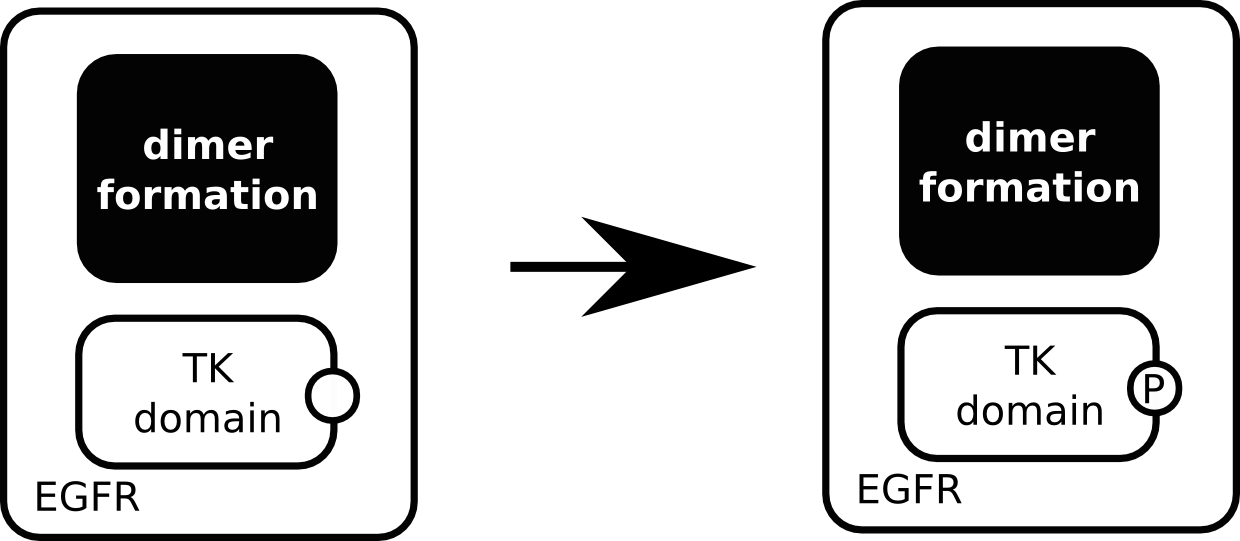
\includegraphics[scale=0.9]{figs/pngs/phosphorylation.png}

\begin{example}
<!-- -------------------------------------------------------------------------------- -->
<!-- Phosphorylation of EGFR if dimerized                                             -->
<!-- -------------------------------------------------------------------------------- -->

       <reaction id="phosphorylation" reversible="false" fast="false"> 
        <listOfReactants>
          <speciesReference id="react_signal" species="signal" stoichiometry="1">
            <multi:listOfSpeciesRestriction>
              <multi:speciesRestriction multi:id="sr_DimerNonPhosSignal" 
                                        multi:speciesTypeInstance="DimerNonPhosSignal" />
            </multi:listOfSpeciesRestriction>
          </speciesReference>
        </listOfReactants>
        <listOfProducts>
          <multi:productSpeciesReference species="signal" stoichiometry="1">
            <multi:listOfSpeciesRestriction>
              <multi:speciesRestriction multi:id="sr_DimerPhosSignal" 
                                        multi:speciesTypeInstance="DimerPhosSignal />
            </multi:listOfSpeciesRestriction>
          </multi:productSpeciesReference>
        </listOfProducts>

        <multi:reactionRule multi:id="EGFRboundSite">
          <multi:listOfConditions>
            <multi:speciesTypeRestrictionReference multi:speciesTypeRestriction="sr_DimerNonPhosSignal"/>
          </multi:listOfConditions>
          <multi:listOfResults>
            <multi:speciesTypeRestrictionReference multi:speciesTypeRestriction="sr_DimerPhosSignal"/>
          </multi:listOfResults>
            <kineticLaw>
              <math xmlns="http://www.w3.org/1998/Math/MathML" >
                <apply>
                  <times />
                  <ci> kcat </ci>
                  <ci> sr_DimerNonPhosSignal </ci>
                  <ci> intracellular </ci>
                </apply>
              </math>
              <listOfLocalParameters>
                <localParameter id="kcat" value="1">
              </listOfLocalParameters>
            </kineticLaw>
          </multi:reactionRule>

      </reaction>
\end{example}

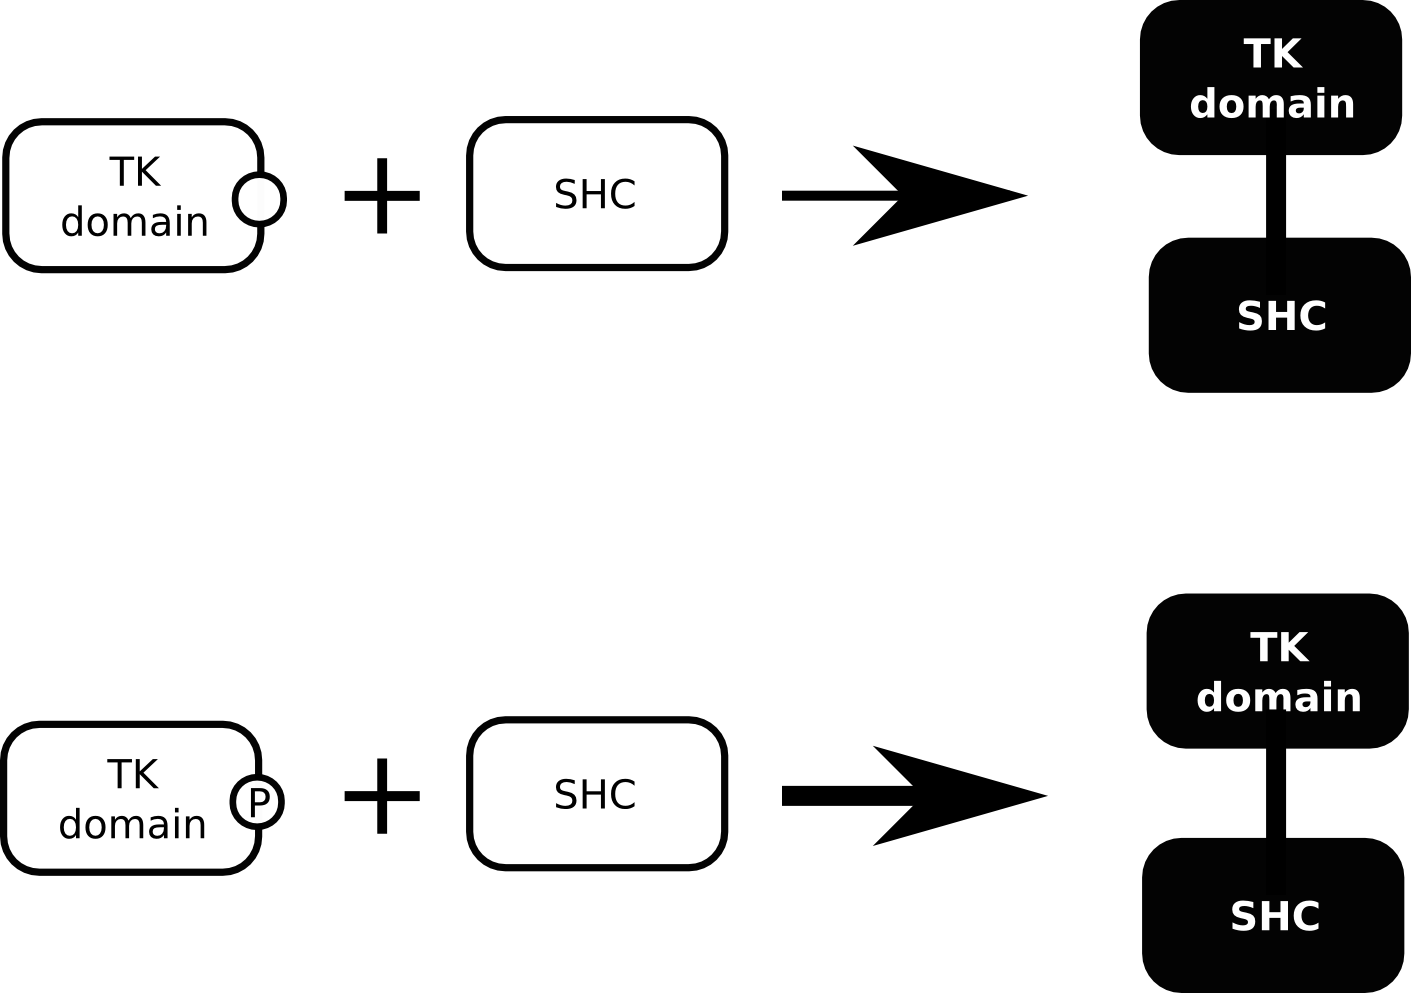
\includegraphics[scale=0.9]{figs/pngs/SHCbinding.png}

\begin{example}
<!-- -------------------------------------------------------------------------------- -->
<!-- SHC binds to EGFR faster if the receptor is phosphorylated                       -->
<!-- -------------------------------------------------------------------------------- -->

       <reaction id="SHCbinding" reversible="false" fast="false"> 
        <listOfReactants>
          <speciesReference id="react_signal" species="signal" stoichiometry="1">
            <multi:listOfSpeciesRestriction>
              <multi:speciesRestriction multi:id="sr_freePhosSignal" 
                                        multi:speciesTypeInstance="freePhosSignal" />
              <multi:speciesRestriction multi:id="sr_freeNonPhosSignal" 
                                        multi:speciesTypeInstance="freeNonPhosSignal" />
            </multi:listOfSpeciesRestriction>
          </speciesReference>
          <speciesReference id="react_SHC" species="SHC" stoichiometry="1">
            <multi:listOfSpeciesRestriction>
              <multi:speciesRestriction multi:id="sr_freeSHC" 
                                        multi:speciesTypeInstance="freeSHC" />
            </multi:listOfSpeciesRestriction>
          </speciesReference>
        </listOfReactants>
        <listOfProducts>
          <multi:productSpeciesReference species="signal" stoichiometry="1">
            <multi:listOfSpeciesRestriction>
              <multi:speciesRestriction multi:id="sr_boundSignal" 
                                        multi:speciesTypeInstance="boundSignal" />
            </multi:listOfSpeciesRestriction>
          </multi:productSpeciesReference>
          <multi:productSpeciesReference species="SHC" stoichiometry="1">
            <multi:listOfSpeciesRestriction>
              <multi:speciesRestriction multi:id="sr_boundSHC" 
                                        multi:speciesTypeInstance="boundSHC"/>
            </multi:listOfSpeciesRestriction>
          </multi:productSpeciesReference>
        </listOfProducts>

        <multi:reactionRule multi:id="rule_NonPhosSignal">
          <multi:listOfConditions>
            <multi:speciesTypeRestrictionReference multi:speciesTypeRestriction="sr_freePhosSignal"/>
            <multi:speciesTypeRestrictionReference multi:speciesTypeRestriction="sr_freeSHC"/>
          </multi:listOfConditions>
          <multi:listOfResults>
            <multi:speciesTypeRestrictionReference multi:speciesTypeRestriction="sr_boundSignal"/>
            <multi:speciesTypeRestrictionReference multi:speciesTypeRestriction="sr_boundSHC"/>
          </multi:listOfResults>
            <kineticLaw>
              <math xmlns="http://www.w3.org/1998/Math/MathML" >
                <apply>
                  <times />
                  <ci> konNP </ci>
                  <ci> sr_freePhosSignal </ci>
                  <ci> sr_freeSHC </ci>
                  <ci> intracellular </ci>
                </apply>
              </math>
              <listOfLocalParameters>
                <localParameter id="konNP" value="1">
              </listOfLocalParameters>
            </kineticLaw>
          </multi:reactionRule>

        <multi:reactionRule multi:id="rule_PhosSignal">
          <multi:listOfConditions>
            <multi:speciesTypeRestrictionReference multi:speciesTypeRestriction="sr_freeNonPhosSignal"/>
            <multi:speciesTypeRestrictionReference multi:speciesTypeRestriction="sr_freeSHC"/>
          </multi:listOfConditions>
          <multi:listOfResults>
            <multi:speciesTypeRestrictionReference multi:speciesTypeRestriction="sr_boundSignal"/>
            <multi:speciesTypeRestrictionReference multi:speciesTypeRestriction="sr_boundSHC"/>
          </multi:listOfResults>
            <kineticLaw>
              <math xmlns="http://www.w3.org/1998/Math/MathML" >
                <apply>
                  <times />
                  <ci> konP </ci>
                  <ci> sr_freeNonPhosSignal </ci>
                  <ci> sr_freeSHC </ci>
                  <ci> intracellular </ci>
                </apply>
              </math>
              <listOfLocalParameters>
                <localParameter id="konP" value="10">
              </listOfLocalParameters>
            </kineticLaw>
          </multi:reactionRule>

      </reaction>

    </listOfReactions>

  </model>
</sbml>
\end{example}
